\documentclass[review]{elsarticle}
%\documentclass[5p]{elsarticle}

\usepackage{lineno,hyperref,gensymb,multirow}
\usepackage[textwidth=18cm]{geometry}
\modulolinenumbers[5]

\journal{Environmental Modelling \& Software}



%%%%%%%%%%%%%%%%%%%%%%%
%% Elsevier bibliography styles
%%%%%%%%%%%%%%%%%%%%%%%
%% To change the style, put a % in front of the second line of the current style and
%% remove the % from the second line of the style you would like to use.
%%%%%%%%%%%%%%%%%%%%%%%

%% Numbered
%\bibliographystyle{model1-num-names}

%% Numbered without titles
%\bibliographystyle{model1a-num-names}

%% Harvard
%\bibliographystyle{model2-names.bst}\biboptions{authoryear}

%% Vancouver numbered
%\usepackage{numcompress}\bibliographystyle{model3-num-names}

%% Vancouver name/year
\usepackage{numcompress}\bibliographystyle{model4-names}\biboptions{authoryear}

%% APA style
%\bibliographystyle{model5-names}\biboptions{authoryear}

%% AMA style
%\usepackage{numcompress}\bibliographystyle{model6-num-names}

%% `Elsevier LaTeX' style
%\bibliographystyle{elsarticle-num}
%%%%%%%%%%%%%%%%%%%%%%%

% Figure sizes:  https://www.elsevier.com/authors/author-schemas/artwork-and-media-instructions/artwork-sizing

\begin{document}
	
\begin{frontmatter}
	
	\title{AtmoSwing: Analog Technique Model for Statistical Weather forecastING and downscalING}
	
	
	\author[unibe,unil,terranum]{Pascal Horton\corref{correspondingauthor}}
	\cortext[correspondingauthor]{Corresponding author}
	\ead{pascal.horton@giub.unibe.ch}
	
	
	\address[unibe]{University of Bern, Oeschger Centre for Climate Change Research, Institute of Geography, Bern, Switzerland}
	\address[unil]{University of Lausanne, Institute of Earth Sciences, Lausanne, Switzerland}
	\address[terranum]{Terranum SARL, Bussigny, Switzerland}
	
	
	
	\begin{abstract}
		Analog methods (AMs) allow for the prediction of local meteorological variables of interest (predictand) such as the daily precipitation, on the basis of synoptic variables (predictors). They can rely on outputs of numerical weather prediction models in the context of operational forecasting or outputs of climate models in the context of climate impact studies. AMs require low computing capacity and have demonstrated a useful potential for application in several contexts. 
		
		AtmoSwing is an open source software written in C++ that implements AMs in a flexible manner so that different variants can be handled dynamically. It comprises four tools: a Forecaster that performs operational forecasts, a Viewer for displaying the results, a Downscaler for climate studies, and an Optimizer for inferring the relationship between the predictand and predictors. It provides valuable results, as revealed by a three-year-long operational forecast in the Swiss Alps. 
	\end{abstract}
	
	\begin{keyword}
		Analog Method; Precipitation; Downscaling; Forecasting
	\end{keyword}
	
\end{frontmatter}

\linenumbers


\section{Introduction}

Approaches based on the concept of analogy are widespread in different domains of science and engineering. In hydrometeorology, it entails retrieving data on atmospheric conditions from the past that can be considered as similar to the situation at hand, with consequences that may be expected to be similar. The consequences can be local variables of interest such as the occurrence of fog, favorable conditions for avalanches, wind intensity, or the precipitation amount. The approach relies on the idea expressed by \citet{Lorenz1956, Lorenz1969}, that similar situations in terms of atmospheric circulation are likely to lead to similar local weather. The approach requires at least two concurrent archives: one describing the situation through different variables called predictors, and another one that provides the value of the local variable of interest called the predictand. 

Usually, the predictand values could be derived by modeling the chain of processes linking the predictors to the predictand. The processes involved range from large-scale dynamical states of the atmosphere down to very small-scale microphysical processes. These require models that are extremely complex, data-intensive, and time-consuming. Conversely, given an appropriate set of predictor archives, a sufficient number of situations analogous to a target situation could be identified so that reasonable values will be obtained for the predictand, at a reasonable coding and computing-time cost. This is particularly true for a specific predictand that is critical in hydrometeorological applications, namely, the precipitation amount over a given domain and time duration. Incidentally, the forecast is proposed as a statistical distribution based on the values assumed by the predictand in the set of analogs selected, unless only the single best analog is considered, which may not prove to be the most efficient \citep{Bontron2005}.

Analog methods (AMs) are used in two different types of approaches \citep{Rummukainen1997}: perfect prognosis, for which the statistical relationship is calibrated based on observed predictors, and model output statistics (MOS), for which the relationship is calibrated against the outputs of a specific climate or numerical weather prediction (NWP) model. AMs are often used to predict daily precipitation, either in an operational forecasting context \citep[e.g.][]{Guilbaud1997, Bontron2005, Hamill2006, Bliefernicht2010, Marty2012, Horton2012, Hamill2015, BenDaoud2016} or a climate downscaling context \citep[e.g.][]{Zorita1999, Wetterhall2005, Wetterhall2007, Matulla2007, Radanovics2013, Chardon2014, Dayon2015, Raynaud2016b}. Other predictands are also considered, such as precipitation radar images \citep{Panziera2011,Foresti2015a}, temperature \citep{Radinovic1975, Woodcock1980, Kruizinga1983, DelleMonache2013, Caillouet2016, Raynaud2016b}, wind \citep{Gordon1987, DelleMonache2013, DelleMonache2011, Vanvyve2015, Alessandrini2015, Junk2015, Junk2015c}, solar radiation or power production \citep{Alessandrini2015a, Bessa2015, Raynaud2016b}, snow avalanches \citep{Obled1980, Bolognesi1993}, and the trajectory of tropical cyclones \citep{Keenan1981, Sievers2000, Fraedrich2003}. \citet{Guilbaud1997} performed a literature review on the use of the AM in long-term forecasting and identified operational applications for monthly forecasts in many countries, including Canada \citep{Shabbar1986},  Hungary \citep{Toth1989}, the Netherlands \citep{Nap1981}, and England \citep{Murray1974}, as well as seasonal forecasts: \citet{Barnett1978}, \citet{Bergen1982} and \citet{Livezey1988}.

An AM was evaluated during the project STARDEX \citep[\textit{STAtistical and Regional dynamical Downscaling of EXtremes for European regions}, see][]{Goodess2003, Stardex2005}. One of the goals of the project was to compare various downscaling methods to determine weather extremes, and the AM was selected as being among the most useful based on several techniques \citep{Maheras2005, Schmidli2007}. \citet{Bliefernicht2010} obtained superior results with the AM than downscaling methods based on weather typing.

The use of the AMs for operational forecasting of daily precipitation originates in the work of \citet{Duband1970, Duband1974, Duband1981}. They were then designed for operational forecasting at EDF (Electricit\'{e} de France) in order to better manage water resources and flood risks. They have been used mainly by practitioners, notably hydropower companies \citep{Desaint2008a, BenDaoud2009, Obled2014} or flood forecasting services in France and Switzerland \citep{Marty2010, GarciaHernandez2009b, Horton2012}. When comparing the results from AMs to an ensemble forecast, \citet{Marty2010} found AMs to be better than the considered ensemble, particularly in the case of strong precipitation. However, AMs should not be considered as a substitute for NWP models, but as a complement in order to obtain a fast and partially independent forecast that is known to be accurate several days in advance. Therefore, they contribute to the analysis of potentially critical situations in flood forecasting, for example, and are very useful in early warning.

\citet{Hamill2006} used an analogy-based approach on the GFS reforecasts in order to correct systematic errors in the ensemble forecasts of temperature and precipitation. These biases could be corrected by taking into account the intrinsic local climatology from the AM. Moreover, the under-dispersion of the ensemble forecast from the numerical model has also been corrected using analogs \citep{Hamill2006}. Correction of ensemble forecast under-dispersion using AMs is also utilized operationally at EDF (\'{E}lectricit\'{e} de France).

The present work does not introduce a new method, but instead, a software called AtmoSwing that implements AMs in a versatile and efficient way. It is versatile in that it facilitates the building of AM structures in a dynamic way with XML files, and because the code is written with an object-oriented architecture. It is efficient because it is written in C++ and leverages parallel computing. AtmoSwing is made up of different modules targeted either for operational forecasting (the Forecaster and the Viewer) or for climate impact studies (the Downscaler). Additionally, a module is available for calibrating the different parameters required for the method, namely the Optimizer. AtmoSwing is continuously evolving and has been used in \citet{Horton2012, Horton2017a, Horton2017b, Horton2018a} and \citet{Horton2018b}.

Some existing AMs designed for daily precipitation will first be described along with the required data (Sect. \ref{sec:data_methods}) and the software will then be presented (Sect. \ref{sec:atmoswing}) together with the details of the modules: the Forecaster (Sect. \ref{sec:forecaster}), the Viewer (Sect. \ref{sec:viewer}), the Downscaler (Sect. \ref{sec:downscaler}), and the Optimizer (Sect. \ref{sec:optimizer}). The conclusion (Sect. \ref{sec:conclusions}) includes some additional perspectives for future developments of AtmoSwing. 


\section{Data and methods}
\label{sec:data_methods}


\subsection{Required data}
\label{sec:data}

AMs generally require three datasets: the historical predictand values, the historical predictor values for the same period and the predictors describing the target situation.

The predictand is often a daily time series. It can have a higher temporal resolution such as 6 hours, but not higher than the time step of the predictors. The most used predictand is the daily precipitation, which is usually averaged over subregions in order to smooth local effects \citep{Obled2002, Marty2012}. These time series are frequently normalized by the precipitation value for a return period of 10~years \citep{Djerboua2001}. This normalization allows for an easier comparison between subregions subject to different precipitation regimes, and thus to better identify the most important contributions.

In the early days when the method was first used, the predictors were based on radio sounding data. Currently, the predictors' archive is often a global atmospheric reanalysis dataset, which provides gridded large-scale variables at any location in the world. Reanalyses are produced using a single version of a data assimilation system coupled with a forecast model constrained to follow observations over a long period. They provide multivariate outputs that are physically consistent, which contain information on the locations where few or no observations are available, including variables that are not directly observed \citep{Gelaro2017}. Even though reanalyses are considered as very accurate in a data-rich region such as Europe, they can have a non-negligible impact on the skill of the prediction, that can be even higher than the choice of the predictor variables \cite{Dayon2015, Horton2018b}. AtmoSwing can read ten different reanalyses (Table \ref{table:datasets}), and others can be easily added due to the encapsulation of the dataset characteristics in the objects. Users can find recommendations for the selection of a reanalysis in \cite{Horton2018b}. Other predictor archives can also be used such as Sea Surface Temperature \citep[SST, ][]{Reynolds2007}. \citet{Bontron2004} proposed that the minimum length of the archive should be 30 years for the prediction of usual conditions, and 40 years or more for intense events.

\begin{table*}[hbt!]
	\caption{Reanalysis datasets that can be read by AtmoSwing.}
	\begin{center}
		\begin{tabular}{ccccccc}
			\hline
			\multirow{2}{*}{\textbf{Name}} & \multirow{2}{*}{\textbf{Institution}} & \textbf{Period} & \textbf{Output} & \textbf{Model} & \textbf{Model} & \textbf{Type of}\\ 
			&& \textbf{of record} & \textbf{resolution} & \textbf{resolution} & \textbf{vintage} & \textbf{input} \\ 
			\hline 
			\textbf{NR-1} & NCEP, NCAR & 1948 -- present & 2.5\degree x 2.5\degree & T62 ($\sim$1.88\degree), L28 & 1995 & full \\
			\textbf{NR-2} & NCEP, DOE & 1979 -- present & 2.5\degree x 2.5\degree & T62 ($\sim$1.88\degree), L28 & 2001 & full \\
			\textbf{ERA-INT} & ECMWF & 1979 -- present & 0.75\degree x 0.75\degree & TL255 ($\sim$0.70\degree), L60 & 2006 & full \\
			\textbf{20CR-2c} & NOAA-CIRES & 1851 -- 2014 & 2\degree x 2\degree & T62 ($\sim$1.88\degree), L28 & 2008 & surface \\
			\textbf{CFSR} & NCEP & 1979 -- present & 0.5\degree x 0.5\degree & T382 ($\sim$0.31\degree), L64 & 2009 & full \\
			\textbf{JRA-55}  & JMA & 1958 -- present & 1.25\degree x 1.25\degree & TL319 ($\sim$0.36\degree), L60 & 2009 & full \\
			\textbf{JRA-55C}  & JMA & 1958 -- 2015 & 1.25\degree x 1.25\degree & TL319 ($\sim$0.36\degree), L60 & 2009 & conventional \\
			\textbf{ERA-20C} & ECMWF & 1900 -- 2010 & 1\degree x 1\degree & TL159 ($\sim$1.13\degree), L91 & 2012 & surface \\
			\textbf{MERRA-2} & NASA GMAO & 1980 -- present & 0.625\degree x 0.5\degree & 0.625\degree x 0.5\degree, L72 & 2014 & full \\ 
			\textbf{CERA-20C} & ECMWF & 1901 -- 2010 & 1\degree x 1\degree & T159 ($\sim$1.13\degree), L91 & 2016 & surface \\
			\hline 
		\end{tabular} 
	\end{center}
	\label{table:datasets}
\end{table*}

The predictors’ dataset that describes the target situation varies according to the application of the AM. For operational forecasting (Sect. \ref{sec:forecaster}) they are outputs of NWP models such as the European Centre for Medium--Range Weather Forecasts (ECMWF) Integrated Forecasting System (IFS) or the National Centers for Environmental Prediction's (NCEP) Global Forecast System \citep[GFS,][]{Kanamitsu1991,Kanamitsu1989}. For climate impact studies (Sect. \ref{sec:downscaler}), they are outputs of general circulation models (GCMs) or regional climate models (RCMs), such as the Coupled Model Intercomparison Project Phase 5 \citep[CMIP5,][]{Taylor2012} and EURO-CORDEX \citep{Jacob2014}.


\subsection{Analog methods for daily precipitation}
\label{sec:method}

AtmoSwing does not rely on a single variant of the AM, but instead can implement different variants. A non-exhaustive selection will be presented hereafter, focusing on the prediction of daily precipitation. Some of these are more specific for a certain region and may not be relevant to others. In addition, some perform better depending on the lead time.


\subsubsection{Characteristics of the AM}

\textit{Definition of the analogy} -- The AM is based on the principle that two similar synoptic situations may produce similar local effects \citep{Lorenz1956}. The perfect analogy does not exist, but sufficiently similar situations leading to similar effects can be identified. Thus, two states of the atmosphere that are alike are called analogs \citep{Lorenz1969}. To be relevant, this analogy must be selected by optimizing the following elements:

\begin{itemize}		
	\item The meteorological variables (predictors) must contain synoptic scale information with a direct or indirect dependency with the target predictand.
	\item The pressure level, or height, at which the predictor is selected.
	\item The spatial window is the domain over which predictors are compared. The ideal size of this area is that which maximizes the useful information and minimizes noise.
	\item The temporal window is the hour(s) of the day for which the predictors are considered.
	\item The analogy criterion required to compare the variables on the chosen spatial and temporal windows is a distance measure used to rank observed situations according to their degree of similarity with the target situation.
	\item Eventual weights between the predictors \cite[e.g.,][]{Horton2017b, Junk2015}.
	\item The optimal number of analog situations $N_{i}$ for the level $i$ which is the best compromise to take into account local variability and maximize useful synoptic information.
\end{itemize}

\textit{Seasonal preselection} -- \citet{Lorenz1969} restricted the search for analog situations to the same period of the year to cope with seasonal effects. This preselection is now often implemented as a moving selection of $\pm$60~days centered around the target date, for every year of the archive (Table \ref{table:methods}). Alternatively, the candidate dates can be selected based on similar air temperature at the nearest grid point \citep[Table \ref{table:methods}][]{BenDaoud2016}.

\begin{table*}[h]
	\caption{Some existing analog methods, listed by increasing complexity. P0 is the preselection (PC: on calendar basis, that is $\pm 60$ days around the target date), L1, L2 and L3 are the subsequent levels of analogy. N1, N2 and N3 are the number of analogs to select at each level of analogy. The meteorological variables are: Z -- geopotential height, T -- air temperature, W -- vertical velocity, MI -- moisture index, which is the product of the relative humidity at the given pressure level and the total water column, MF -- moisture flux, which is the product of MI with the wind intensity. The analogy criterion is S1 for Z and RMSE for the other variables.}
	\begin{center}
		\begin{tabular}{ccccccccl}
			\hline
			\textbf{Type} & \textbf{P0} & \textbf{L1} & \textbf{N1} & \textbf{L2} & \textbf{N2} & \textbf{L3} & \textbf{N3} & \textbf{Reference} \\ 
			\hline 
			\textbf{PC-2Z} & PC & Z1000@12h & 50 &&&&& \citealt{Bontron2004} \\
			&& Z500@24h &&&&&& \\
			\hline 
			\textbf{PC-4Z} & PC & Z1000@06h & {\raise.17ex\hbox{$\scriptstyle\sim$}}27 &&&&& \citealt{Horton2018a} \\
			&& Z1000@30h &&&&&& \\
			&& Z700@24h &&&&&& \\
			&& Z500@12h &&&&&& \\
			\hline 
			\textbf{PC-2Z-2MI} & PC & Z1000@12h & 70 & MI850@12h & 30 &&& \citealt{Bontron2004} \\
			&& Z500@24h && MI850@24h &&&& \\
			\hline 
			\textbf{PC-2Z-2MI} & PC & Z1000@06h & 75 & MI925@06h & 30 &&& \citealt{Marty2010} \\
			&& Z500@18h && MI925@18h &&&& \\
			\hline 
			\textbf{PC-2Z-2MF} & PC & Z1000@06h & 60 & MF700@06h$^{\dagger}$ & 25 &&& \citealt{Marty2010} \\
			&& Z500@18h && MF700@18h &&&& \\
			\hline 
			\textbf{PC-4Z-2MI} & PC & Z1000@30h & {\raise.17ex\hbox{$\scriptstyle\sim$}}63 & MI700@24h & {\raise.17ex\hbox{$\scriptstyle\sim$}}24 &&& \citealt{Horton2018a}\\
			&& Z850@12h && MI600@12h &&&& \\
			&& Z700@24h &&&&&& \\
			&& Z400@12h &&&&&& \\
			\hline 
			\textbf{PT-2Z-4MI} & T925@36h & Z1000@12h & 70 & MI925@12h & 25 &&& \citealt{BenDaoud2016} \\
			& T600@12h & Z500@24h && MI925@24h &&&& \\
			&&&& MI700@12h &&&& \\
			&&&& MI700@24h &&&& \\
			\hline 
			\textbf{PT-2Z-10MI} & T925@36h & Z1000@12h & 70 & MI925@06-30h & 25 &&& \citealt{BenDaoud2010} \\
			& T600@12h & Z500@24h && MI700@06-30h &&&& \\
			\hline 
			\textbf{PT-2Z-4W-4MI} & T925@36h & Z1000@12h & 170 & W850@06h & 70 & MI925@12h & 25 & \citealt{BenDaoud2016} \\
			& T600@12h & Z500@24h && W850@12h && MI925@24h && \\
			&&&& W850@18h && MI700@12h && \\
			&&&& W850@24h && MI700@24h && \\
			\hline 
		\end{tabular} 
	\end{center}
	
	$\dagger$ or MF925@06h+18h as an alternative
	\label{table:methods}
\end{table*}
\clearpage

\textit{Analogy of atmospheric circulation} -- A conditioning by variables describing the atmospheric circulation is present in a vast majority of AMs. The geopotential field (Z) is often used as a predictor since \citet{Lorenz1969}, who based the analogy on the levels 200, 500, and 850~hPa. Several pressure levels were later assessed by means of various criteria for the analogy based on the geopotential field \citep{Duband1970, Duband1974, Duband1981, Guilbaud1997}. It was determined to be important to calculate the analogy for multiple pressure levels and different temporal windows (time of observation) instead of a unique selection \citep{Guilbaud1998, Obled2002}. \citet{Bontron2004} showed that the choice of the temporal window plays a greater significance compared to the choice of the atmospheric level for the performance of the AM for daily precipitations. He concluded that the coupled geopotential heights at 1000~hPa (Z1000) at 12~h~UTC and 500~hPa (Z500) at 24~h~UTC provided the best performance \citep[for a subset of the NCEP/NCAR Reanalysis I;][]{Kalnay1996, Kistler2001} for the investigated regions in France (Table \ref{table:methods}). The analogy for the atmospheric circulation proposed by \citet{Bontron2004} is still used operationally at the time of writing. \citet{Marty2010} tested other temporal windows for intraday application on the basis of a more comprehensive reanalysis dataset and proposed to change the hours of observation to 06~h and 18~h. \citet{Horton2018a} showed that a selection of four combinations of pressure levels and temporal windows instead of two for the geopotential height improves the prediction skill (PC-4Z, Table \ref{table:methods}). The pressure levels and temporal windows were automatically selected by genetic algorithms for the upper Rhone catchment in Switzerland.

\textit{Additional levels of analogy} -- Additional levels of analogy are subsequent steps that subsample a lower number of analog situations from the antecedent level of analogy, based on other variables. A second level of analogy was first introduced by \citet{Mandon1985}, \citet{Vallee1986}, and \citet{Gibergans-Baguena2007}, based on wind, moisture variables, stability indexes, or temperature. After a systematic assessment, \citet{Bontron2004} noted that a moisture index (MI) based on the product of the relative humidity at 850~hPa (RH850) and the total precipitable water (TPW) gave the best performance (Table \ref{table:methods}). This index does not represent an actual physical quantity, but expresses the water content of the air column and its degree of saturation. \citet{Marty2010} selected the MI at 925~hPa instead of 850~hPa and also considered the moisture flux (MF) at 700 or 925~hPa (Table \ref{table:methods}). The MF is the product of the MI with the wind intensity. \citet{Horton2018a} determined that MI at 600 and 700~hPa were more useful than MF after the circulation analogy was applied to the four atmospheric levels (Table \ref{table:methods}). \citet{BenDaoud2016} also reconsidered the parameters of MI and ended up with both 925~hPa and 700~hPa levels (Table \ref{table:methods}). Subsequently, they added an additional level of analogy between the circulation and the moisture analogy (Table \ref{table:methods}) based on the vertical velocity at 850~hPa (W850). This AM, termed "SANDHY" for Stepwise Analogue Downscaling method for Hydrology \citep{BenDaoud2016, Caillouet2016}, was primarily developed for large and relatively flat/lowland catchments in France (Sa\^{o}ne, Seine).

\textit{Analogy criteria} -- In early applications of AMs, the geopotential height was condensed using principal component analysis (PCA) and the selection of analog situations was performed according to a Euclidean distance in the space of the PCA, which was eventually combined with a correlation criterion in order to remove days that are close in distance but too dissimilar in pattern. \citet{Guilbaud1997} stopped using PCA to work directly with the raw data interpolated on grids, which resulted in an improvement. In the case of the variables that describe atmospheric circulation, the Teweles--Wobus (S1) criterion \citep[Eq. (\ref{eq:S1}), ][]{Teweles1954, Drosdowsky2003} was identified as the most suited criteria based on different studies \citep{Wilson1980, Woodcock1980, Guilbaud1998, Bontron2004}. S1 allows for a comparison of the gradients and thus an analogy of the atmospheric circulation instead of a Euclidean distance. For other predictors, the classic criteria representing absolute distances are used: Mean Absolute Error (MAE) and Root Mean Squared Error (RMSE), the latter being used most often.

\begin{equation}
\label{eq:S1}
S1=100 \frac {\displaystyle \sum_{i} \vert \Delta\hat{z}_{i} - \Delta z_{i} \vert}
{\displaystyle \sum_{i} max\left\lbrace \vert \Delta\hat{z}_{i} \vert , \vert \Delta z_{i} \vert \right\rbrace }
\end{equation}
where $\Delta \hat{z}_{i}$ is the forecast geopotential height difference between the \textit{i}th pair of adjacent points from the grid of the target situation, and $\Delta z_{i}$ is the corresponding observed geopotential height difference in the candidate situation. The differences are processed separately in both directions. The smaller the S1 values, the more similar the pressure fields.

\textit{Other parameters} -- The predictors are compared for a defined spatial window, which must be optimized to maximize the useful information and minimize noise. The spatial window is usually considered unique for all predictors of a level of analogy. Using genetic algorithms, \citet{Horton2018a} introduced different spatial windows between the pressure levels, which increased performance. Additionally, a weighting between the predictors was also successfully added instead of a simple equal-weights averaging. The number of analogs to select at each level of analogy should be optimized. It depends on the predictor dataset, the size of the spatial window and the length of the archive \citet{Ruosteenoja1988, Vandendool1994}.

\textit{Probabilistic forecast} -- After the last level of analogy, the observed predictand of interest (for example, daily precipitation amount) of the $N_{i}$ resulting dates provide the empirical conditional distribution considered as the probabilistic forecast for the target day. The empirical frequencies are processed for every value of the predictand after classification, based on the Gringorten parameters \cite[for a Gumbel or exponential law; see][]{Gringorten1963} and a probabilistic model can eventually be fitted \citep[e.g. Gamma function,][]{Obled2002}. The forecast is finally often synthesized according to percentiles 20, 60 and 90~\% \citep{Guilbaud1997, Guilbaud1998}.

\textit{Use in operational forecasting} -- In one of the very first uses in operational forecasting, the forecast was performed based only on radiosonde observations and was temporally extrapolated to the two following days. However, because of the chaotic nature of the atmosphere, two analog situations quickly diverge over time \citep{Lorenz1969}. Thus, the AM has strong limitations regarding the temporal extrapolation in operational forecasting \citep{Bontron2004}. Given the superior capability of numerical models for simulating the dynamic evolution of the atmosphere, their outputs are now used as temporal extrapolation of the synoptic variables. The search for analogy thus aims to connect the forecasted synoptic situation with a local predictand (temperature, precipitation, etc.), which is more difficult to simulate for numerical models. When using AMs in operational forecasting, it should be noted that some variables such as moisture or vertical velocity might not be accurately predicted after a lead time of a few days due to higher uncertainties. Predictors describing the atmospheric circulation are generally considered to be more reliable.


\subsubsection{Regional characteristics}

The optimal predictors vary from one region to another, along with the leading atmospheric processes. Thus a unique version of the AM valid for any place on earth cannot be obtained. However, the method needs to be adapted to the local conditions, available data, and to the size of the catchment of interest. Thus, there will always be local adaptations to be made for use in a new region. Even for two locations that are close to each other but subject to different critical atmospheric conditions, the selection of the best predictors can vary. This is illustrated in Fig. \ref{figure:variable_exploration} for two subregions of the Rh\^{o}ne catchment in Switzerland. For both regions, all variables of NR-1 were assessed by optimizing the spatial window and the number of analogs for each one of them using the sequential calibration tool implemented in AtmoSwing (Sect. \ref{sec:vars-explo}). The main similarities in the selection of the best predictor from the NCEP/NCAR reanalysis I at both locations are: (1) the variables describing the atmospheric circulation (pressure fields or geopotential heights) perform best, and (2) they are better when compared with the S1 criteria (asterisk in Fig. \ref{figure:variable_exploration}) instead of the RMSE. The main difference is that the pressure fields better explain the precipitation when they are considered close to the ground for the Chablais region, and at a higher altitude for the South-east crests. This is driven by the elevation of the stations and by the main atmospheric influences related to precipitation events at these locations. 

\begin{figure*}[hbt!]
	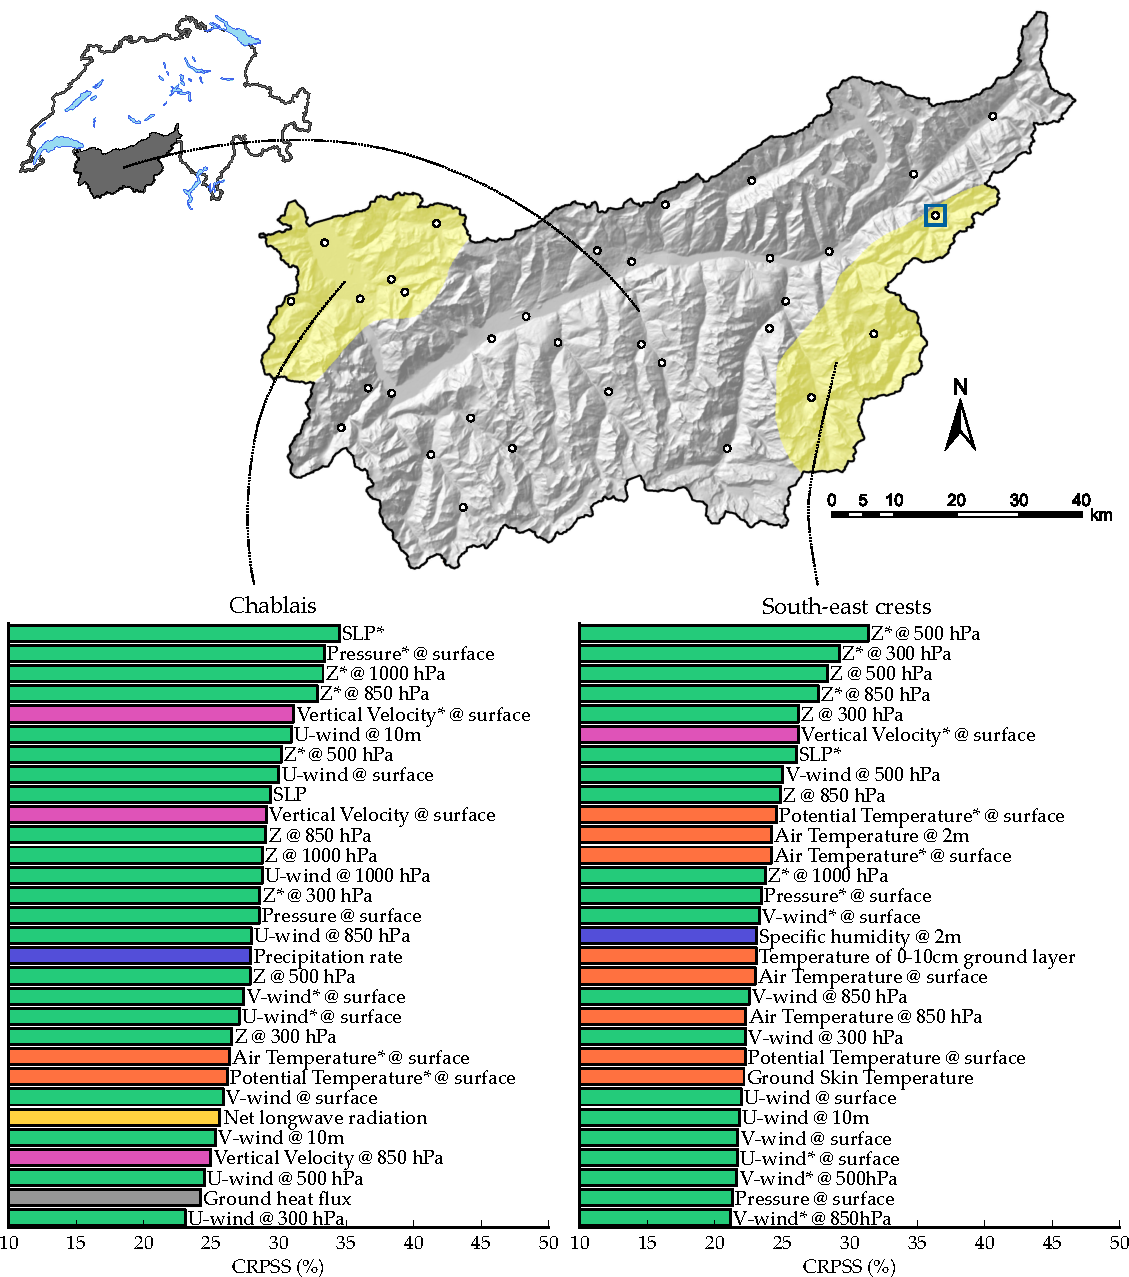
\includegraphics[width=14cm]{figures/fig_01.pdf}
	\caption{Performance score (CRPSS) of the 30 best variables from the NCEP/NCAR reanalysis dataset, when considered separately (no combination), for the Chablais region and the southeast ridges. The analogy criterion is S1 when there is an asterisk next to the variable name, and RMSE otherwise. Colour illustrates the variable type: green = atmospheric circulation, blue = moisture, orange = temperature, yellow = radiation, purple = vertical velocity, and gray = other. SLP stands for sea level pressure and Z for geopotential height. The blue square indicates the Binn station, which is analyzed in more detail later on.} 
	\label{figure:variable_exploration}
\end{figure*}

The choice of the best predictors is likely to vary from one reanalysis dataset to another. This comprehensive comparison was not repeated with other datasets, because a selection of the best predictors using genetic algorithms would be less cumbersome (Sect. \ref{sec:global-optimization}).


\subsubsection{Method nomenclature}

Variants of the AMs are numerous and it is not always easy to reference them in a short and descriptive way. In AtmoSwing, a basic nomenclature is used (Fig. \ref{figure:nomenclature}) in order to express the structure into a simple identifier. This cannot describe all the parameters of the AM, but quickly illustrates the structure of the implementation. This is particularly useful when working with a global optimization method, where nothing is fixed but the structure of the AM. This nomenclature has been used in \citet{Horton2017a, Horton2017b, Horton2018a} and \citet{Horton2018b}.

\begin{figure}[hbt!]
	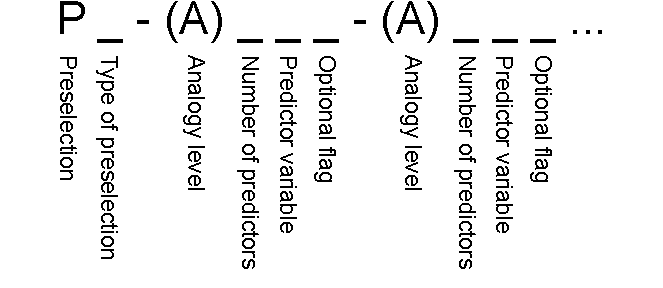
\includegraphics[width=9cm]{figures/fig_02.pdf}
	\caption{Proposed structure for naming the parameterizations of the AM.}
	\label{figure:nomenclature}
\end{figure}

The naming contains different blocs (separated by a hyphen) for the various levels of analogy. It starts with the specification of the preselection (P; can be omitted when comparing AMs with the same preselection approaches), which can be one of two types:
\begin{itemize}
	\item PC: calendar period ($\pm 60$ days around the target date)
	\item PT: based on air temperature \citep{BenDaoud2010}
\end{itemize}

Then, the following levels of analogy are listed, which may start with an optional A (for analogy). For every level of analogy, the number of variables used (combination of atmospheric levels and time of observation) is first provided, and then the short name of the variable is given (according e.g. to ECMWF conventions; in upper case), for example:
\begin{itemize}
	\item Z: geopotential (circulation)
	\item TPW: total precipitable water
	\item RH: relative humidity
	\item V: wind velocity
	\item W: vertical velocity
	\item MI: moisture index (TPW * RH)
	\item MF: moisture flux (V * TPW * RH)
\end{itemize}

In order to keep the identifier simple, no value of atmospheric level or time of observation is specified. Moreover, the analogy criterion is not specified and is supposed to be S1 for Z and RMSE for the other variables. If anything changes from these conventions, it can be noted as a flag. The flag (lower case) can also provide other information, such as the optimization method:
\begin{itemize}
	\item sc : sequential calibration (can be omitted as considered as default, see Sect. \ref{sec:optimizer})
	\item go (or just ''o''): global optimization (by means of genetic algorithms for example)
\end{itemize}

This nomenclature can be adapted to specific needs or simplified for better readability (e.g. by removing the specification of the preselection). Examples can be found in Table \ref{table:methods}.


\section{AtmoSwing}
\label{sec:atmoswing}

AtmoSwing is made of 4 main modules that are standalone, but do share a common code basis: the Forecaster for operational forecasting, the Viewer for displaying the forecast in a GIS environment, the Downscaler for climate applications, and the Optimizer that is used to infer the statistical relationship that defines the analogy for a given predictand time series. Separating the Forecaster and the Viewer allows for automation of the forecast on a server and the local display of the results. The Forecaster, the Downscaler and the Optimiser can be used either with a graphical user interface or a command-line interface.


\subsection{Technical aspects}

The code is written in object-oriented C++ and relies on the wxWidgets \citep{Smart2006} library to provide a cross-platform native experience to users. CMake is used to build AtmoSwing in MS Windows, Linux / Unix, or Mac (macOS). Developments have been partly performed using a test-driven development (TDD) approach. Continuous integration has been set up so that a collection of more than 600 tests can be evaluated every time new code is pushed to the server, to prevent regressions. Every analogy criterion, prediction score, searching and sorting functions, data manipulation, etc., were tested. Some tests specific to the AM rely on the results of another analog sorting software developed at the Universit\'{e} Grenoble Alpes. They ensure that the results of AtmoSwing are exactly equivalent to this model, given the same parameters and data. The source code is under version control (Git) and is open source \citep[on GitHub, www.atmoswing.org,][]{Horton2018c}. The GitHub organization page (https://github.com/atmoswing) also contains toolboxes to work with the outputs of AtmoSwing in R \citep{Horton2018d} or Python \citep{Horton2018e}.

Although processing an analog prediction for a given target date is fast, hindcasts over periods of several decades must be performed for calibration, which may become very time-consuming. Thus, great effort has been focused on minimizing the processing time using profiling tools. Firstly, all identified redundancies in the processing are removed. Then, when searching for a certain date or data, the search initially occurs in the region where it is likely to be found instead of exploring an entire array. Similar data are not loaded twice, but instead shared pointers are used. Several other improvements allow reducing the computing time, for example the use of the quicksort method \citep{Hoare1962a} to sort the date vectors according to the analogy criterion. Different implementation variants were tested in order to select the most efficient approach: for example, when storing analog dates according to their criterion value, it is faster to insert them in a fixed-size array instead of storing them all and subsequently sorting the array. When using the S1 criteria, the gradients are pre-processed on the predictor data, so that they are only processed once. AtmoSwing also uses the linear algebra library Eigen 3 \citep{Guennebaud2010} for calculations on vectors and matrices, which result in time-saving. Multi-threading is also implemented so that the search for analog situations in the archive is distributed among the available threads. 

A user interface allows for the creation of the predictand database in the NetCDF format from text files. During the process, Gumbel adjustments are automatically calculated for precipitation data to determine the values corresponding to different return periods. The time series are normalized using a selected return period (default 10~years) and their square root can be processed. The final database file contains both the raw and the normalized series, as well as characteristics of the gauging stations and some metadata.


\subsection{Modular approach and implementation}

AtmoSwing's great strength is that it is designed to process the analog method in a modular fashion. The structure of the AM (number of analogy levels, number of predictors) is built dynamically (Fig. \ref{figure:flowchart_modules_atmoswing}), and nothing is fixed a priori. The software then successively performs as many analogy levels as the user specifies, using all the predictors indicated. Each level of analogy results in an object containing target dates, analog dates, values of the analogy criteria, values of the predictand (at the final stage), and other data. This object can be saved as a NetCDF file and/or can be injected into a new analogy level. The whole structure of the AM is defined through an XML file. Even the time step of the method (6 or 24~hours for example) is a dynamic parameter.

\begin{figure}[hbt!]
	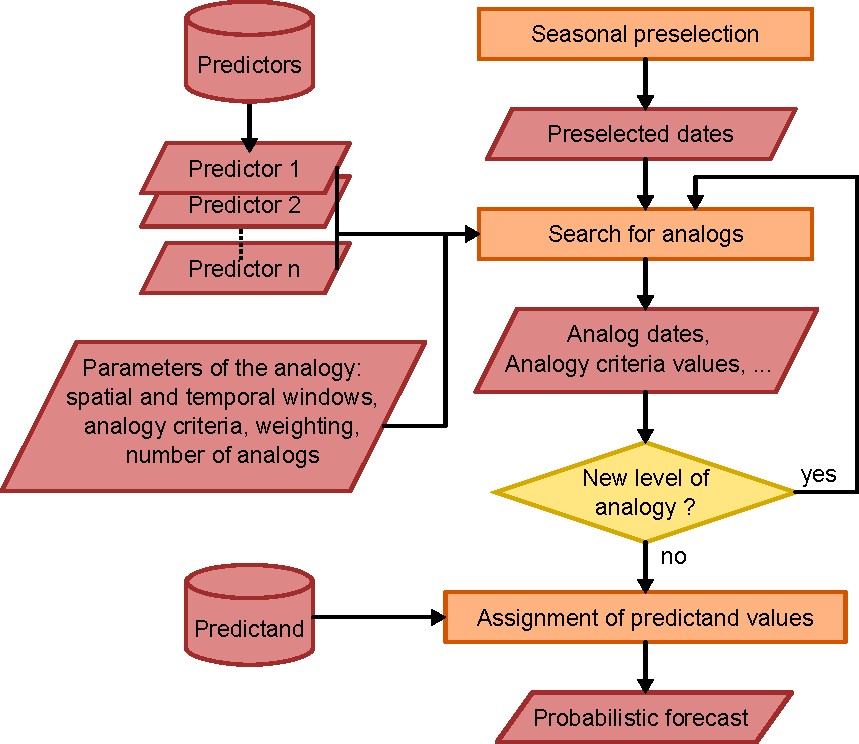
\includegraphics[width=9cm]{figures/fig_03.pdf}
	\caption{Simplified flowchart of the AM implementation in AtmoSwing.}
	\label{figure:flowchart_modules_atmoswing}
\end{figure}

Each implementation of the AM (see Sect. \ref{sec:method}) may enter this scheme, even if it consists of pre-processed variables (e.g. moisture index). Various pre-processing functions are implemented as the calculation of the moisture index or flux, multiplication operations, or calculation of the gradients. The user can dynamically specify the pre-processing method and the predictors to use in the XML file.

This modular approach is implemented through object-oriented programming, as a direct consequence of polymorphism. This allows, for example, processing of a predictor object as a single interface to entities representing any reanalysis dataset. Similarly, the criterion can be of different types, as well as the score for calibrating. Figure \ref{figure:code_diagram} illustrates the main classes or objects involved in the core of the analog method processing in AtmoSwing in a simplified way. The different types of objects that are instantiated are defined in the XML parameters file. Thus, there is a single implementation of the analog method capable of interacting with different object types in various contexts (calibration, forecasting, downscaling). 

\begin{figure*}[hbt!]
	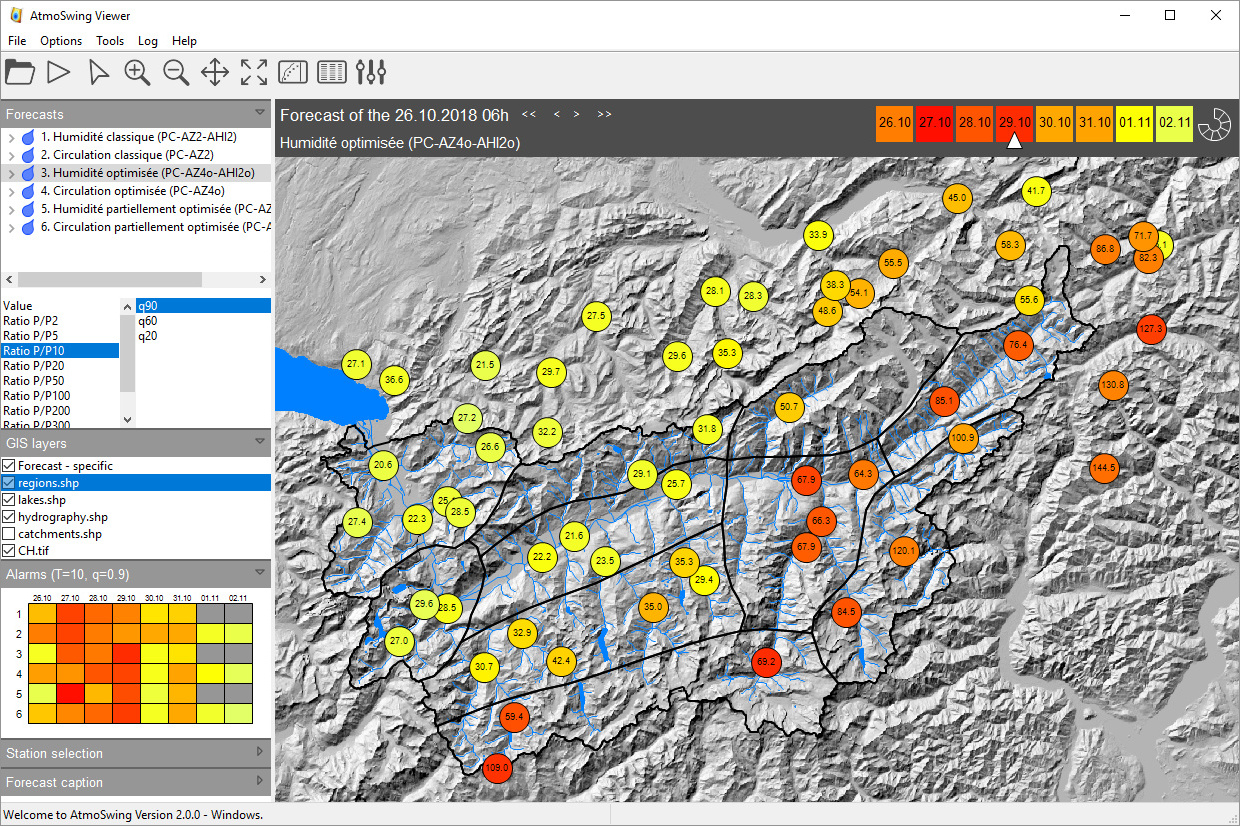
\includegraphics[width=19cm]{figures/fig_04.pdf}
	\caption{Simplified illustration of the main classes or objects involved in the core of the AM processing in AtmoSwing. The processor class interacts with parent classes that can represent different entities, such as different reanalysis datasets, predictand, criteria, scores, and in different contexts: calibration, forecasting, and downscaling. The items in green are only available in the Optimizer, the ones in blue, in the Forecaster, and the ones in Orange, in the Downscaler. The area represents the spatial window and the time array a list of candidate dates (from preselection or previous analogy levels). The links to the parameters illustrate the dynamic definition of the different types by the parameters from the XML file.}
	\label{figure:code_diagram}
\end{figure*}


\subsection{AtmoSwing Forecaster}
\label{sec:forecaster}

The Forecaster module allows processing of operational forecasts. The software can be compiled with a graphical user interface (GUI), or without it to be used on a headless server through a command line interface (CLI). Processing a forecast requires very low computing capabilities and can be performed on a low-end computer. It successfully runs on a Raspberry Pi 3 (Model B).

To this day, the software can use the outputs of IFS or GFS (see Sect. \ref{sec:data}). When using GFS, it first downloads the predictor describing the target situation. It then linearly interpolates the gridded data to match the resolution of the archive. The analogs dates are next extracted according to the selected AM variant and the predictand data are associated with the corresponding dates. The results are finally saved in auto-describing NetCDF files. If requested, a synthetic XML file is generated for easier integration on a web platform, for example. Every step of the forecast, from predictor downloading (when possible) to the final results, is performed in the software (and controlled through configuration), without the use of external scripts (e.g. for data conversion).

Both the GUI and the CLI facilitate a forecast based on the most recent NWP outputs, or for a given date or period. When there is no new predictor data available, the forecast is not processed and computing resources are not utilized. The recommended use is thus to set up an automatic task on a server to trigger the forecast every 30 minutes. This would for example provide four forecasts a day. 

Before being used in operational forecasting, the AMs were calibrated in a perfect prognosis framework, usually using a reanalysis dataset (Sect. \ref{sec:optimizer}). However, this does not take into account the uncertainty related to the forecast of the target situation by Numerical Weather Prediction models. One might be willing to take into account this uncertainty, which increases with the lead time. A solution is to increase the number of analog situations with the lead time, which should be optimized for every lead time on a forecast archive or a reforecast dataset \citep{Thevenot2004}. This technique is available in AtmoSwing, as the number of analogs can be specified for every lead time.

A meteorological variable that was proven as a good predictor in the perfect prognosis framework may eventually be poorly predicted by the selected NWP beyond a certain lead time. It should then be dropped after this lead time. For example, when using moisture variables for the second level of analogy, \citet{Thevenot2004} showed that beyond a lead time of three days the AM with two levels did not perform better than the one with a single level of analogy. Datasets of reforecast from the selected NWP models allow assessing these aspects for different lead times.


\subsection{AtmoSwing Viewer}
\label{sec:viewer}

AtmoSwing Viewer allows for the display of the files produced by the Forecaster in an interactive GIS environment (Fig. \ref{figure:atmoswing-viewer-gui}). It provides several levels of synthesis of the forecasts. It first provides an overview of possible alerts using color codes on the lead time switcher (upper right in the GUI, see Fig. \ref{figure:atmoswing-viewer-gui}) that represent the worst case scenarios, or in the alarm panel (on the left side of the GUI). The alarm panel allows for a synthesis of the highest forecasted values for the different AMs and the different lead times. By default, the colors are expressed relative to the 10~year return period, for the $90^{th}$ percentile (which can be changed in the preferences). This highest level of synthesis allows for quick identification of potentially critical situations in the days ahead.

\begin{figure*}[hbt!]
	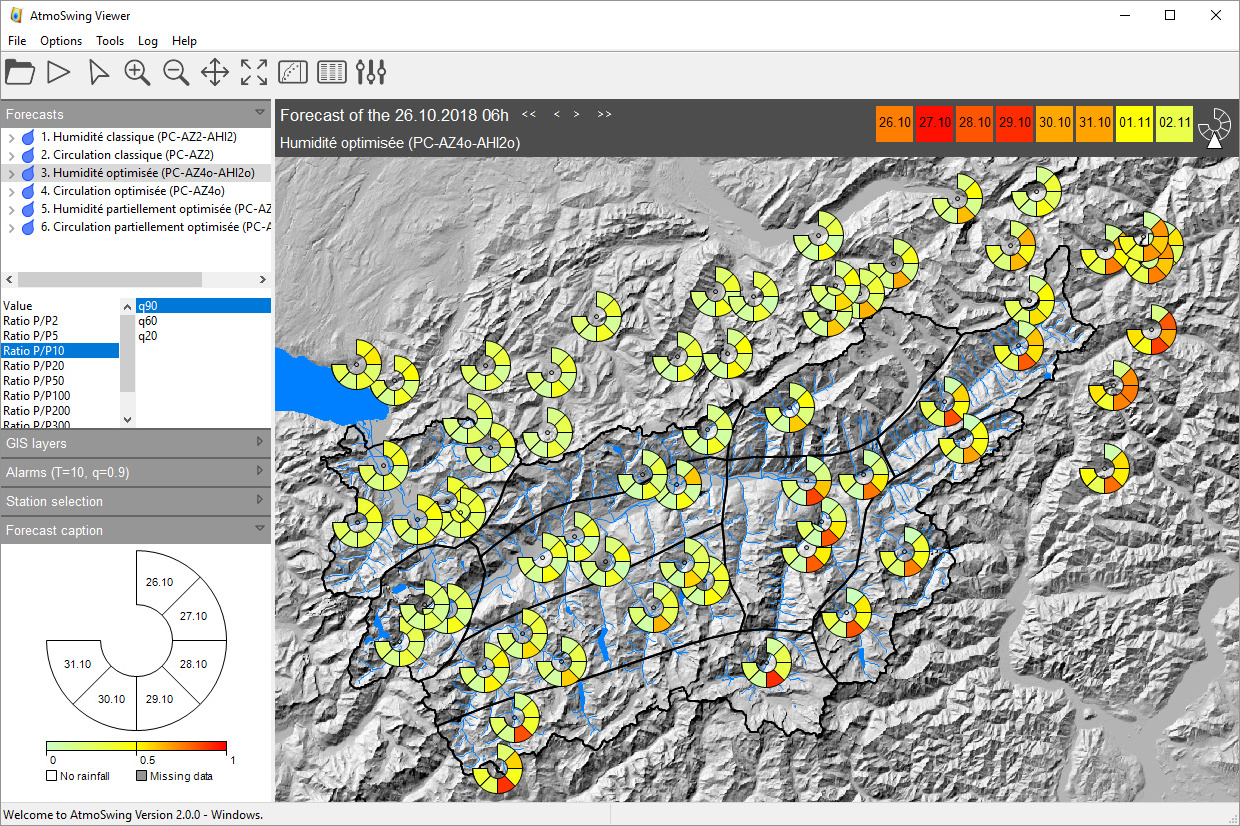
\includegraphics[width=19cm]{figures/fig_05.jpg}
	\caption{Graphical user interface of the Viewer module (Elevation data from The Shuttle Radar Topography Mission (SRTM), and hydrological network from SwissTopo).}
	\label{figure:atmoswing-viewer-gui}
\end{figure*}

Then, the user can explore the forecasts in more details, starting from the provided map (Fig. \ref{figure:atmoswing-viewer-gui}). The map displays the forecast of the selected AM variant (selected in the upper left panel) and the selected lead time (upper right). During the forecast, one AM might have parameters that differ by subregions, such as the number of analogs or the spatial windows. The Viewer automatically gathers the similar AM types and provides a composite view of the optimal forecasts per subregion. The user can, however, choose to display the results associated with a single parameter set for the entire region (by opening the tree view and selecting a child element), which provides a homogeneous set of analog dates. A display of all lead times on a single map is possible based on a symbolic representation on a circular band with a box for every lead time (Fig. \ref{figure:atmoswing-viewer-snail}). The number of boxes is adjusted to the number of lead times. This representation offers a global spatiotemporal visualization for a chosen AM.

\begin{figure*}[hbt!]
	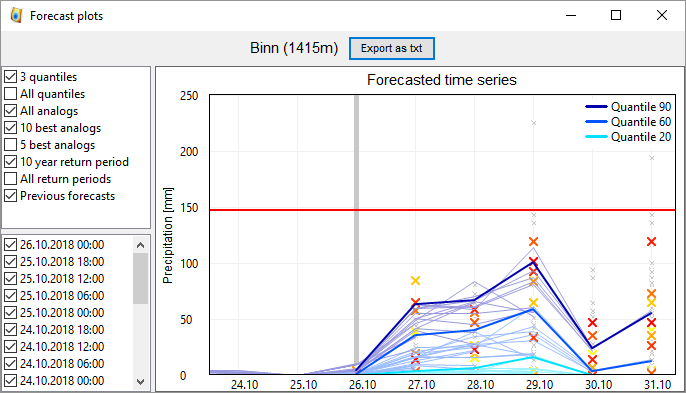
\includegraphics[width=19cm]{figures/fig_06.jpg}
	\caption{Visualization of multiple lead times on the map (Elevation data from the SRTM, and hydrological network from SwissTopo).}
	\label{figure:atmoswing-viewer-snail}
\end{figure*}

Color scales in the map can be adjusted by choosing (on the left part of the GUI) the predictand reference (raw value or ratio to different return periods) and the quantile of the distribution. Using a ratio to a certain return period eases the interpretation of the expected precipitation given that reference volumes can drastically differ from one location to another, particularly in mountainous regions. All information relative to a rain gauge station (or catchment), such as its location, its name, or the values of different return periods, are stored in the forecast files to be displayed for end users who do not have the predictand database.

By clicking on a station on the map (or by selection from a dropdown list on the left), a new window appears with a plot of the forecasted time series (Fig. \ref{figure:atmoswing-viewer-timeseries}). By default, the plot contains the usual three considered percentiles (90$^{th}$, 60$^{th}$, and 20$^{th}$), along with the 10 best analogs with a color code from yellow (tenth) to red (first). The 10-year return period value is also displayed to set the perspective of the forecast. The user can choose to hide any data or to display supplementary information (all analogs, all 10$^{th}$ percentiles, or all return periods) in the left panel. Traces of previous forecasts are also automatically loaded and displayed to provide information on the consistency of the forecasts. 

\begin{figure}[hbt!]
	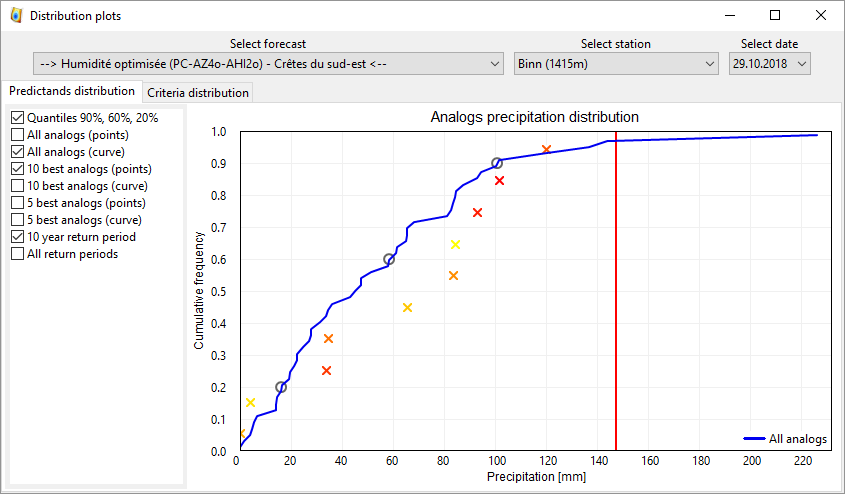
\includegraphics[width=9cm]{figures/fig_07.png}
	\caption{Visualization of the forecasted time series for an event at the Binn station (Fig. \ref{figure:variable_exploration}) in October 2018.}
	\label{figure:atmoswing-viewer-timeseries}
\end{figure}

The user can then delve into further details and display the predictand cumulative distribution for a given lead time (Fig. \ref{figure:atmoswing-viewer-distribution}). This can inform if there is a shift between the distribution of all analogs versus the 10 best. Such a shift warns of a risk of under/overestimation when considering the full distribution, particularly for high precipitation amounts. Indeed, the number of extreme precipitation events in the archive is limited and they are thus likely to be underrepresented in the selected analog dates. Different authors have shown that if the 60$^{th}$ percentile is best to forecast the occurrence and the amount of precipitation for common situations, the 90$^{th}$ percentile is a better indicator for strong to extreme events \citep{Djerboua2001, Bontron2004, Marty2010}. It is, therefore, necessary to pay close attention when the 90$^{th}$ percentile reaches high values, as this may be indicative of possible extreme precipitations due the presence of several analog dates with high precipitation amounts in the distribution \citep{Djerboua2001}.

\begin{figure}[hbt!]
	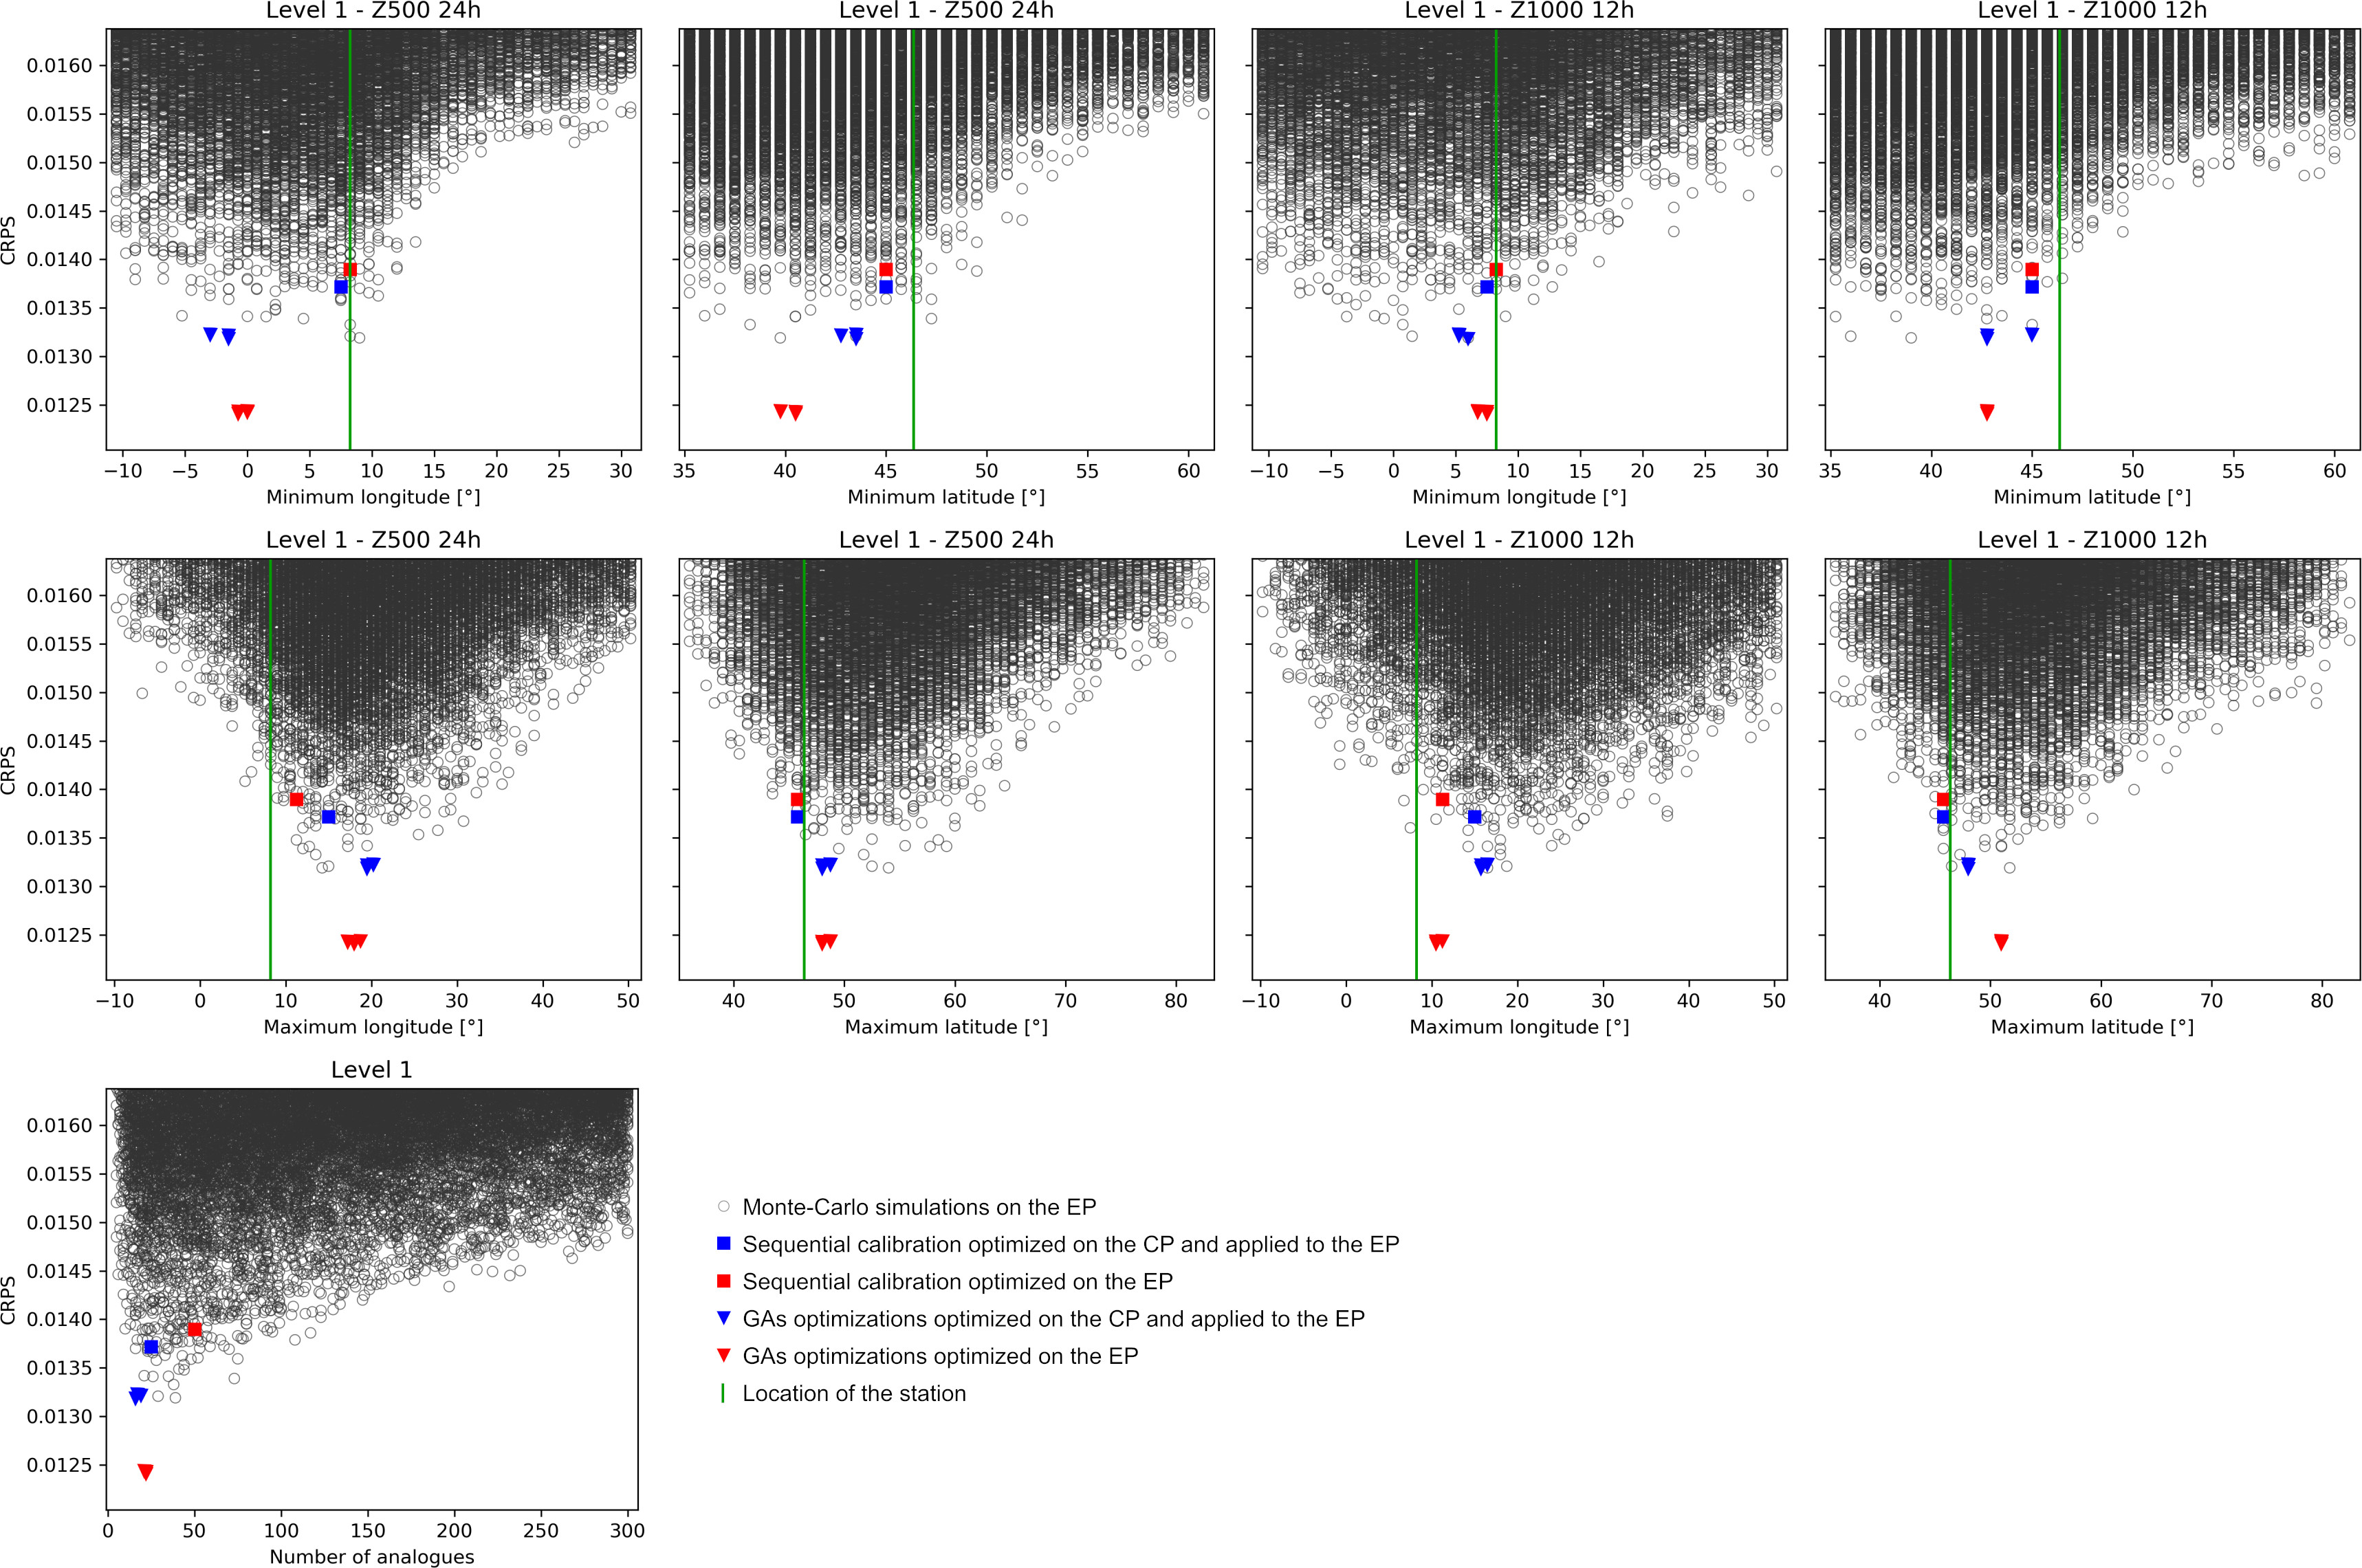
\includegraphics[width=9cm]{figures/fig_08.png}
	\caption{Visualization of the forecasted precipitation distribution for a given lead time for an event at the Binn station (Fig. \ref{figure:variable_exploration}) in October 2018.}
	\label{figure:atmoswing-viewer-distribution}
\end{figure}

The distribution of the analogy criteria (not shown) can also be displayed to identify eventual discontinuities in the criteria values. Finally, one can display a grid containing the analog dates with the corresponding predictand and criteria values in an interactive spreadsheet (not shown). 

AtmoSwing Viewer relies on workspaces defined in XML files to specify the path to the forecast directories and the GIS layers. It is thus easy to switch from a forecast for a region to another. Many GIS formats are supported thanks to GDAL \cite[Geospatial Data Abstraction Library,][]{GDAL2014}. A user can have as many layers as desired and can control their display properties (color, transparency).


\subsection{AtmoSwing Downscaler}
\label{sec:downscaler}

The Downscaler module is the last addition to AtmoSwing. Its purpose is to downscale either climate model outputs for climate impact studies or reanalyses for climate reconstruction of the past. 

The Downscaler is able to read outputs of general circulation models (GCMs) or regional climate models (RCMs), such as the Coupled Model Intercomparison Project Phase 5 \citep[CMIP5,][]{Taylor2012} and EURO-CORDEX \citep{Jacob2014}, and can be extended to other datasets. CMIP5 and EURO-CORDEX are distributed in the NetCDF format, but present a great variety of time steps, temporal references, spatial resolution, and file structures. A complete redesign of the management of the predictor data was necessary to provide the flexibility required to account for this variety. The Downscaler is thus able to parse these datasets original files by exploiting the self-descriptive capacity of NetCDF files. 

The use of AMs in the context of future climate is new. Not all AMs can be used for this purpose, because some predictors might not capture the climate change signal well and the preservation of the relationship between predictors and predictands must prevail. However, several authors have demonstrated the transferability of some AMs for future climate \citep{Dayon2015, Dayon2018, Raynaud2016, Turco2017}. The transferability of an AM must be assessed before it is used in such a context. 

AMs have also been used to perform climate reconstruction of the past \citep{Caillouet2016, Caillouet2017, Bonnet2017}. Such applications allow, for example, hydrological modeling of flood events in periods where no meteorological data are available, or analysis of past severe droughts. 


\subsection{AtmoSwing Optimizer}
\label{sec:optimizer}

AtmoSwing Optimizer is a single tool that integrates different optimization methods, presented in Sect. \ref{sec:sequential} to \ref{sec:global-optimization}. Its purpose is to infer the statistical relationship between the predictors and a predictand. The calibration framework is detailed in Sect. \ref{sec:calibration-framework} and the implemented skill scores are listed in Sect. \ref{sec:scores}.


\subsubsection{Calibration framework}
\label{sec:calibration-framework}

The calibration of the AM is usually performed in a perfect prognosis \citep{Klein1959} framework \citep{Bontron2004, BenDaoud2010}. Perfect prognosis uses observed or reanalyzed data to calibrate the relationship between predictors and predictands, as opposed to the MOS approach that establishes the relationship based on model outputs. As a result, perfect prognosis yields relationships that are as close as possible to the natural links between predictors and predictands. However, there are no perfect models and even reanalysis data may contain bias that cannot be ignored \citep{Dayon2015, Horton2018b}. Thus, the considered predictors should be as robust as possible, i.e., they should have minimal dependence on the model. With MOS approaches, reforecasts can be used to establish the relationship between predictors and predictands, provided that the archive is long enough. However, the calibration procedure must be performed every time a new version is available in order to reduce the bias \citep{Wilson2002}.

A statistical relationship is inferred with a trial and error approach by processing a forecast for every day of a calibration period. A certain number of days close to the target date are excluded to consider only independent candidate days. Validating the parameters of AMs on an independent validation period is very important to avoid over-parametrization and to ensure that the statistical relationship is valid for another period. In order to account for climate change and the evolution of measuring techniques, it is recommended that a noncontinuous period for validation should be used, distributed over the entire archive \citep{BenDaoud2010, Horton2018b}. AtmoSwing's users can thus specify a list of the years to set apart for the validation that are removed from possible candidate situations. At the end of the optimization, the validation score is processed automatically.


\subsubsection{Implemented performance scores}
\label{sec:scores}

Multiple scores are implemented in AtmoSwing Optimizer and are listed hereafter. Details are only provided for the CRPS \citep[Continuous Ranked Probability Score,][]{Brown1974, Matheson1976, Hersbach2000}, which is most often used. 


\textit{Discrete deterministic predictions} - These are, for example, deterministic predictions of threshold exceedances. The continuous probabilistic nature of an ensemble of analogs can be transformed into a discrete prediction by considering a fixed percentile from the distribution, which is compared to a threshold exceedance of the predictand. On the basis of a contingency table \citep{Wilks2006}, multiple scores can be processed with AtmoSwing:

\begin{itemize}
	\item Proportion correct \citep{Finley1884}
	\item Threat Score \citep{Gilbert1884}
	\item Bias
	\item False Alarm Ratio
	\item Hit Rate or Probability of Detection
	\item False Alarm Rate
	\item Heidke Skill Score \citep{Heidke1926}
	\item Peirce Skill Score \citep{Peirce1884}
	\item Gilbert Skill Score or Equitable Threat Score \citep{Gilbert1884}
\end{itemize}


\textit{Continuous deterministic predictions} - These types of predictions must be evaluated using distance measures. For AMs, the provided distribution is summarized by a chosen percentile, which is compared to the predictand value. Available scores are as follows:

\begin{itemize}
	\item Mean Absolute Error
	\item Root Mean Squared Error
\end{itemize}


\textit{Discrete probabilistic predictions} – In this instance, the probability of occurrence or the probability of belonging to a certain category is considered. The implemented scores are as follows:

\begin{itemize}
	\item Brier Score \citep{Brier1950}
	\item ROC diagram \citep[Relative Operating Characteristic or Receiver Operating Characteristic,][]{Mason1982}
	\item RPS \citep[Ranked Probability Score,][]{Epstein1969}
	\item SEEPS \citep[Stable Equitable Error in Probability Space,][]{Rodwell2010,Rodwell2011}
\end{itemize}


\textit{Continuous probabilistic predictions} - These types of predictions are issued in the form of the expected statistical distribution for a variable, which needs to be compared to an observed value. This is the situation encountered when using multiple analogs from AMs.

Most assessment of AMs performance use the CRPS \citep[Continuous Ranked Probability Score,][]{Brown1974, Matheson1976, Hersbach2000}. It allows for evaluation of the predicted cumulative distribution functions $F(y)$, for example, the precipitation values $y$ associated with the analog situations, compared to the single observed value $y^{0}$ for a day $i$:

\begin{equation}
\label{eq:CRPS}
CRPS_{i} = \int_{0}^{+\infty} \left[ F_{i}(y)-H_{i}(y-y_{i}^{0})\right]^{2} dy
\end{equation}
where $H(y-y_{i}^{0})$ is the Heaviside function that is null when $y-y_{i}^{0}<0$, and has the value 1 otherwise; the better the prediction, the lower the score. This score is now commonly used for the evaluation of continuous variable prediction systems \citep{Casati2008, Marty2010}. It can be decomposed into several indicators also implemented into AtmoSwing Optimizer, such as: reliability -- resolution / uncertainty \citep{Hersbach2000}, or sharpness -- accuracy \citep{Bontron2004}.

Its skill score expression is often used, with the climatological distribution of precipitation as the reference. The CRPSS (\textit{Continuous Ranked Probability Skill Score}) is thus defined as follows \citep{Bradley2011}:

\begin{equation}
\label{eq:CRPSS}
CRPSS = 1-\frac{\overline{CRPS}}{\overline{CRPS}_{clim}}
\end{equation}
where $CRPS_{clim}$ is the CRPS value for the climatological distribution. A better prediction is characterized by an increase in CRPSS.

Finally, the rank diagram \citep{Talagrand1997} and its accuracy as defined by \citet{Candille2005} are also available.


\subsubsection{The sequential calibration}
\label{sec:sequential}

The calibration procedure that we call ''sequential'' or ''classic'' was elaborated upon by \citet{Bontron2004} \cite[see also][]{Radanovics2013, BenDaoud2016}. It is a semi-automatic procedure that optimizes the spatial windows in which the predictors are compared and the number of analogs for every level of analogy. The different analogy levels (e.g. the atmospheric circulation or moisture index) are calibrated sequentially. The procedure consists of the following steps \citep{Bontron2004}:

\begin{enumerate}
	\item Manual selection of the following parameters:
	\begin{enumerate}
		\item Meteorological variable
		\item Pressure level
		\item Temporal window (hour of the day)
		\item Number of analogs 
	\end{enumerate}
	
	\item For every level of analogy:
	\begin{enumerate}
		\item Identification of the most skilled unitary cell (1~point for moisture variables and 4 for the geopotential height when using the S1 criteria) of the predictor data over a large domain. Every point or cell of the full domain is jointly assessed based on the predictors of the current level of analogy.
		\item From this most skilled cell, the spatial window is expanded by successive iterations in the direction of the largest performance gain until no further improvement is possible.
		\item The number of analog situations $N_{1}$, which was initially set to an arbitrary value, is then reconsidered and optimized for the current level of analogy.
	\end{enumerate}
	\item A new level of analogy can then be added based on other variables such as the moisture index at chosen pressure levels and hours of the day. The number of analogs for the next level of analogy, $N_{2}$, is initiated at a chosen value. The procedure starts again from step 2 (calibration of the spatial window and the number of analogs) for the new level. The parameters calibrated for the previous analogy levels are fixed and do not change.
	\item Finally, the numbers of analogs $N_{1}$ and $N_{2}$ for the different levels of analogy are reassessed. This is performed iteratively by varying the number of analogs of each level in a systematic manner. 
\end{enumerate}

The calibration is performed in successive steps for a limited number of parameters with the aim of minimizing/maximizing the chosen objective function. Except for the number of analogs, previously calibrated parameters are generally not reassessed. The benefit of this method is that it is relatively fast, it provides acceptable results, and it has low computing requirements. 

Small improvements were incorporated into this method in AtmoSwing Optimizer, then termed as ''classic+'', by allowing the spatial windows to perform other moves, such as: (1) increase in 2 simultaneous directions, (2) decrease in 1 or 2 simultaneous directions, (3) expansion or contraction (in every direction), (4) shift of the window (without resizing) in 8 directions (including diagonals), and finally (5) all the moves described above, but with a factor of 2, 3, or more. For example, an increase by two grid points in one (or more) direction is assessed. This allows skipping one size that may not be optimal. These supplementary steps often result in spatial windows that are slightly different. The performance gain is rather marginal for reanalyses with a low resolution such as NR-1, but might be more consistent for reanalyses with higher resolutions due to the presence of more local minima.


\subsubsection{Variables exploration}
\label{sec:vars-explo}

The sequential calibration can also be used to explore the variables of a dataset. A list of variables, pressure levels, and temporal windows can be provided and all combinations are assessed through the classic(+) calibration. This functionality facilitates a comparison between the different variables of a dataset while considering the effect of the pressure level and the temporal window. Using this approach, only one variable is assessed at a time, but multiple levels of analogy are possible. Figure \ref{figure:variable_exploration} results from such an analysis of the NR-1 reanalysis. 


\subsubsection{Global optimization}
\label{sec:global-optimization}

The sequential calibration has strong limitations: (i) it cannot automatically choose the pressure levels and temporal windows (hour of the day) for a given meteorological variable, (ii) it cannot handle dependencies between parameters, and (iii) it cannot easily handle new degrees of freedom. For this reason, genetic algorithms (GAs) were implemented in AtmoSwing Optimizer to perform a global optimization of AMs. This allows for optimization of all parameters jointly in a fully automatic and objective way. The method is described in \citet{Horton2017a} and an application is provided in \citet{Horton2018a}.


\subsubsection{Monte--Carlo simulations}
\label{sec:monte-carlo}

A Monte--Carlo analysis is also implemented in AtmoSwing. The procedure performs thousands of assessments of random parameters within given ranges. This method is not efficient for finding the best parameters set, but facilitates a better understanding of the sensitivity of the parameters. Its relevance is however limited for AMs with multiple levels of analogy and variables. Indeed, for methods with a high number of parameters with wide authorized value ranges, the probability is too low to obtain an acceptable configuration, and thus the resulting response surface might not be representative of the actual distribution of optimal values (See examples in Sect. \ref{sec:parameters-space}). 


\section{Parameters space of AMs}
\label{sec:parameters-space}

An analysis of the parameters resulting from Monte--Carlo simulations, the sequential calibration, and GAs was performed for the Binn station in Switzerland (Fig. \ref{figure:variable_exploration}) with ERA-INT (Table \ref{table:datasets}). Binn is characterized by high precipitation totals and heavy rainfall in this region, and on several occasions was responsible for large damages downstream. For this reason, it is a station of particular interest. The results for this station cannot be generalized to all stations, but similar conclusions can be drawn for other locations. Moreover, the parameters space at a single station is expected to be significantly more irregular than averaged regional precipitations.

The analysis was first performed for the 2Z method (Table \ref{table:methods}) for the period 2001--2010 for the target, and 1981--2010 as the archive. A relatively short period of 10 years was chosen to allow for 50,000 Monte--Carlo simulations. The plots in Fig. \ref{figure:monte_carlo_r1} are truncated at the best $25^{th}$ percentile. The Monte--Carlo simulations show that the spatial window for Z needs to cover a certain region, but can be larger than a critical size. The extent of the spatial window can thus be substantially different without significantly affecting the performance score. This was also observed by \citet{Bontron2004}, who noted that ''\textit{performance slowly decreases if we consider a window that is slightly too large, while using windows that are too small results in strong performance loss}''. The dilution of the relevant synoptic information therefore does not necessarily have a significant negative impact on performance, while ignoring some of this information leads to stronger losses of performance. The issue of equifinality related to the spatial windows is discussed in \cite{Radanovics2013}. The station is usually contained within the optimal spatial domain, provided the predictors are considered on the same day as the predictand. The optimal number of analogs is relatively well defined, although the selection of more analog candidates is possible without a strong penalty in terms of performance.

\begin{figure*}[hbt!]
	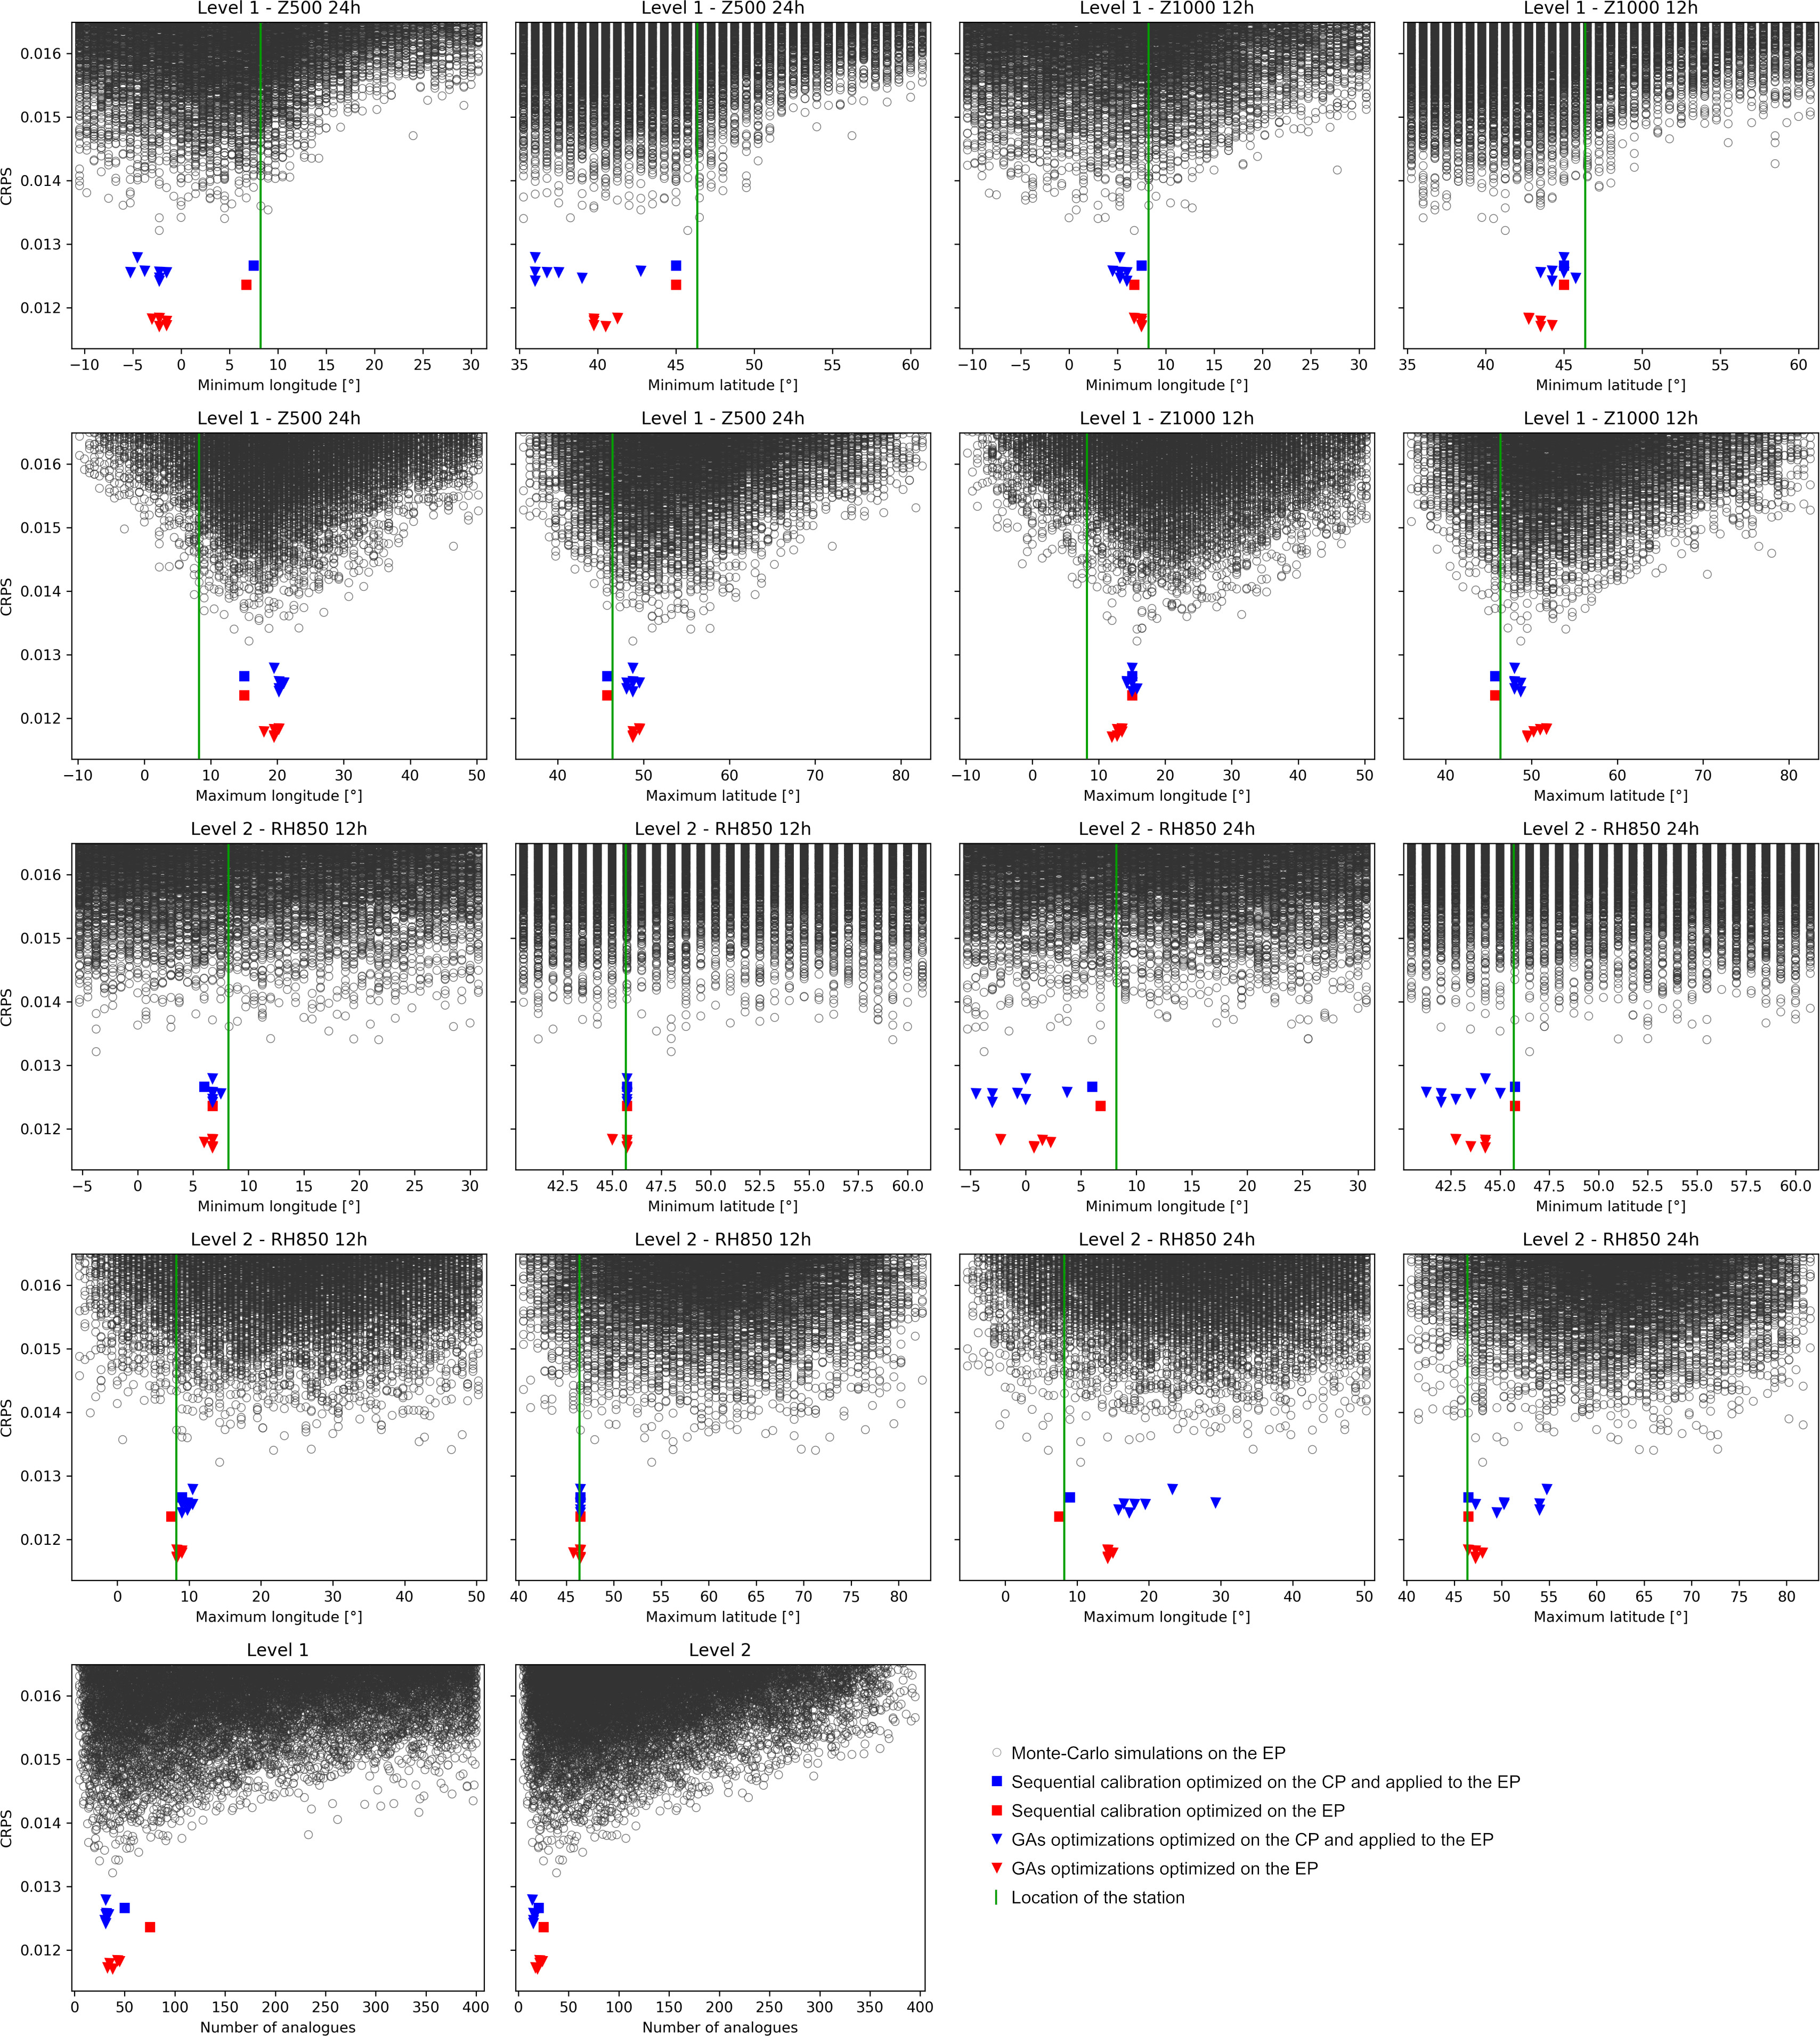
\includegraphics[width=19cm]{figures/fig_09.jpg}
	\caption{Example of parameter values for 2Z (Table \ref{table:methods}) for the precipitation at the Binn station (Fig. \ref{figure:variable_exploration}) on the period 2001--2010. The parameters are the extent (min/max longitude/latitude) of the spatial windows for the geopotential height at 500 and 1000~hPa, and the number of analogs. The green vertical bar in the plots represents the location of the station. The circles represent random parameters from the Monte--Carlo analysis. The plots are truncated at the $25^{th}$ best percentiles for 50,000 realizations. Squares are the results of the sequential calibration and triangles result from genetic algorithms. Markers in blue represent parameters optimized for the period 1981--2000 and applied to 2001--2010. Markers in red represent parameters optimized directly for the period 2001--2010.}
	\label{figure:monte_carlo_r1}
\end{figure*}

The results of the sequential calibration are also illustrated in Fig. \ref{figure:monte_carlo_r1} (with squares). The calibration was first performed for the period 1981--2000 and applied to 2001--2010 (blue squares) but also calibrated directly for the 2001--2010 period (red squares). Here, the parameters established on a different calibration period provided slightly better results. This is due to the limitations of the sequential calibration that can easily be trapped in a local optima. Indeed, the resulting spatial windows are small in this case, and the algorithm stops as soon as an increase of the domain does not improve the score. This might not be an issue with a low-resolution reanalysis such as NR-1 (2.5\degree; Table \ref{table:datasets}), but this might become more of an issue with higher resolutions, such as ERA-INT used here (0.75\degree), because local minima are more frequent. In this case, the classic+ approach (Sect \ref{sec:sequential}) might be relevant. The Monte-Carlo analysis yielded some better parameter sets than the sequential calibration, due to the constraint on the latter to have the same spatial window for both pressure levels. 

Fourteen optimizations by GAs were performed for the same setup (seven optimizations using the 2001--2010 period as validation (blue triangles) and seven optimizations using this period as the calibration period directly (red triangles)). The optimization with GAs was given the same degrees of freedom as the Monte--Carlo simulations, so no weighting of the pressure levels was considered \citep[as in][]{Horton2018a}. Thus, the parameters optimized for the 2001--2010 period (red) could have been found randomly using the Monte--Carlo simulations. However, this did not occur due to the low probability of obtaining this combination. GAs also result in more skillful parameters than the sequential calibration. When optimized for the 2001--2010 period (red triangles), the parameters yielded results that outperform the optimization for the 1981--2000 period (blue triangles). However, the contrary is expected for the later period. Most optimizations converge to a narrow range of values, supposedly, the global optimum for the respective period. The main difference compared to the sequential calibration is that the spatial windows are substantially larger, mainly for Z500, and they differ between pressure levels.  

Monte--Carlo simulations were also performed for 2Z-2MI (Table \ref{table:methods}) for the same periods and for the same station. Figure \ref{figure:monte_carlo_r2} shows that the Monte--Carlo simulations could not properly use the moisture variables of the second level of analogy. The boxplots for the second level of analogy show an indifference of the location and the size of the spatial windows, which is demonstrated to be wrong, based on the other optimization methods. Moreover, the achieved CRPS here based on random parameters is not better than the case without the moisture variables (Fig. \ref{figure:monte_carlo_r1}). Additionally, the number of analogs corresponding to the best CRPS values are similar between the two levels of analogy, which means that the second level is simply discarded. There are too many parameters with acceptable ranges that are too narrow to obtain meaningful parameters randomly. Monte--Carlo simulations with uniform probability laws is not suited for even moderately complex AMs. 

\begin{figure*}[hbt!]
	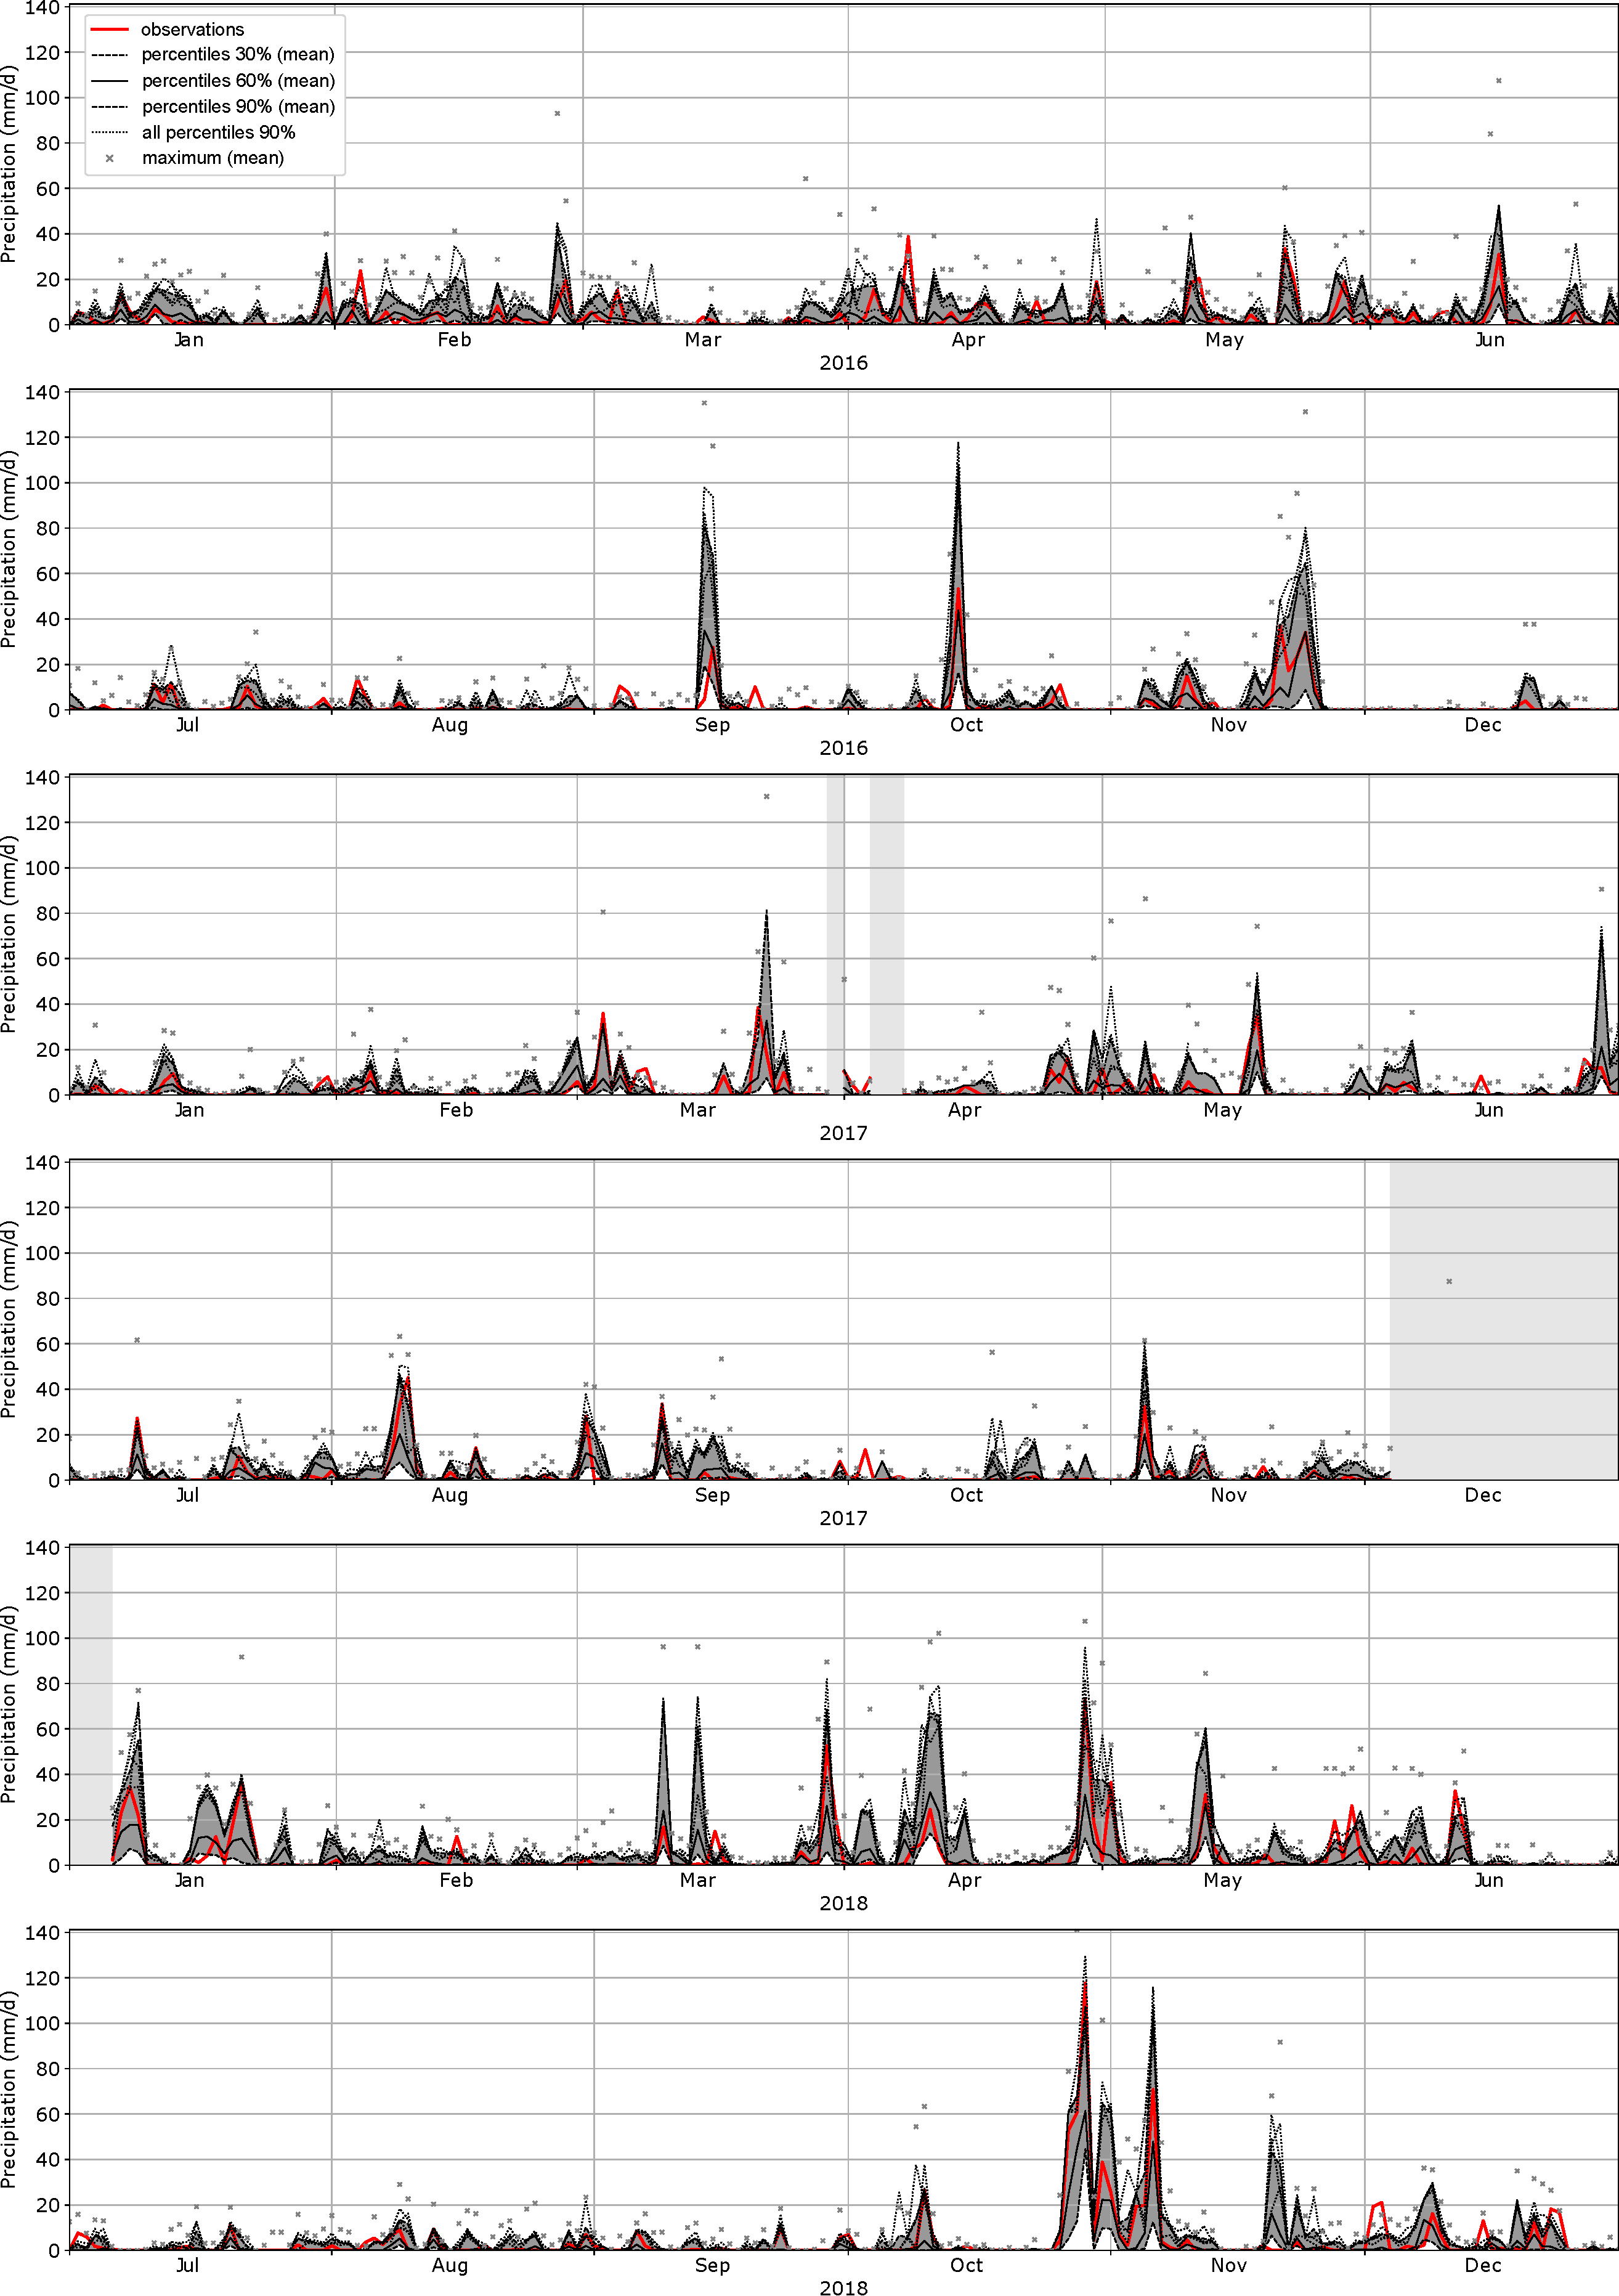
\includegraphics[width=19cm]{figures/fig_10.jpg}
	\caption{Same as Fig. \ref{figure:monte_carlo_r1} but for 2Z-2MI (Table \ref{table:methods}). Results are shown for both levels of analogy (geopotential height and moisture index).}
	\label{figure:monte_carlo_r2}
\end{figure*}
\clearpage

The sequential calibration results in small spatial windows, especially for moisture variables. The differences with the 2Z methods for the first level of analogy are due to the different initial number of analogs, which has an influence on the choice of the spatial windows. The optimized parameters for the 2001--2010 period perform better than the ones established based on the other calibration period, which can be expected.

The results of the GAs show more variability than previously, which is likely due to a higher difficulty related to the larger number of parameters that have to be optimized, and to the presence of potentially more correlated information. The choice of the spatial windows for the moisture index at 12~h~UTC is similar between the different optimization techniques and is a small line of zonally extended points. The chosen spatial windows by GAs for the moisture index at 24~h~UTC is surprisingly large. This is likely due to the search of the GAs for additional information at a more distant location due to highly correlated data between 12~h~UTC and 24~h~UTC at the same 850~hPa level. The lack of convergence for this second spatial window means that the use of this variable is likely not optimal, and it would probably add more information considered at another pressure level, which was shown in \citet{Horton2018a}. The analysis of the convergence of multiple GA optimizations can thus be useful in interpreting the results and in identifying potentially suboptimal structures or variables.

The former results present a relatively noisy signal for the different optimization methods or the Monte--Carlo simulations. This may be due (1) to the fact that we consider a station’s time series instead of regional ones, which could decrease some variability from small-scale patterns in the precipitation fields, and (2) because we consider a short period for calibration. Despite the high number of simulations, Monte--Carlo simulations with a uniform probability law are not appropriate for even moderately complex AMs. It is likely that using a Gaussian probability law centered on the station would be more appropriate.


\section{Feedback from operational forecast}
\label{sec:operational}

\begin{figure*}[hbt!]
	\vspace{-70pt}
	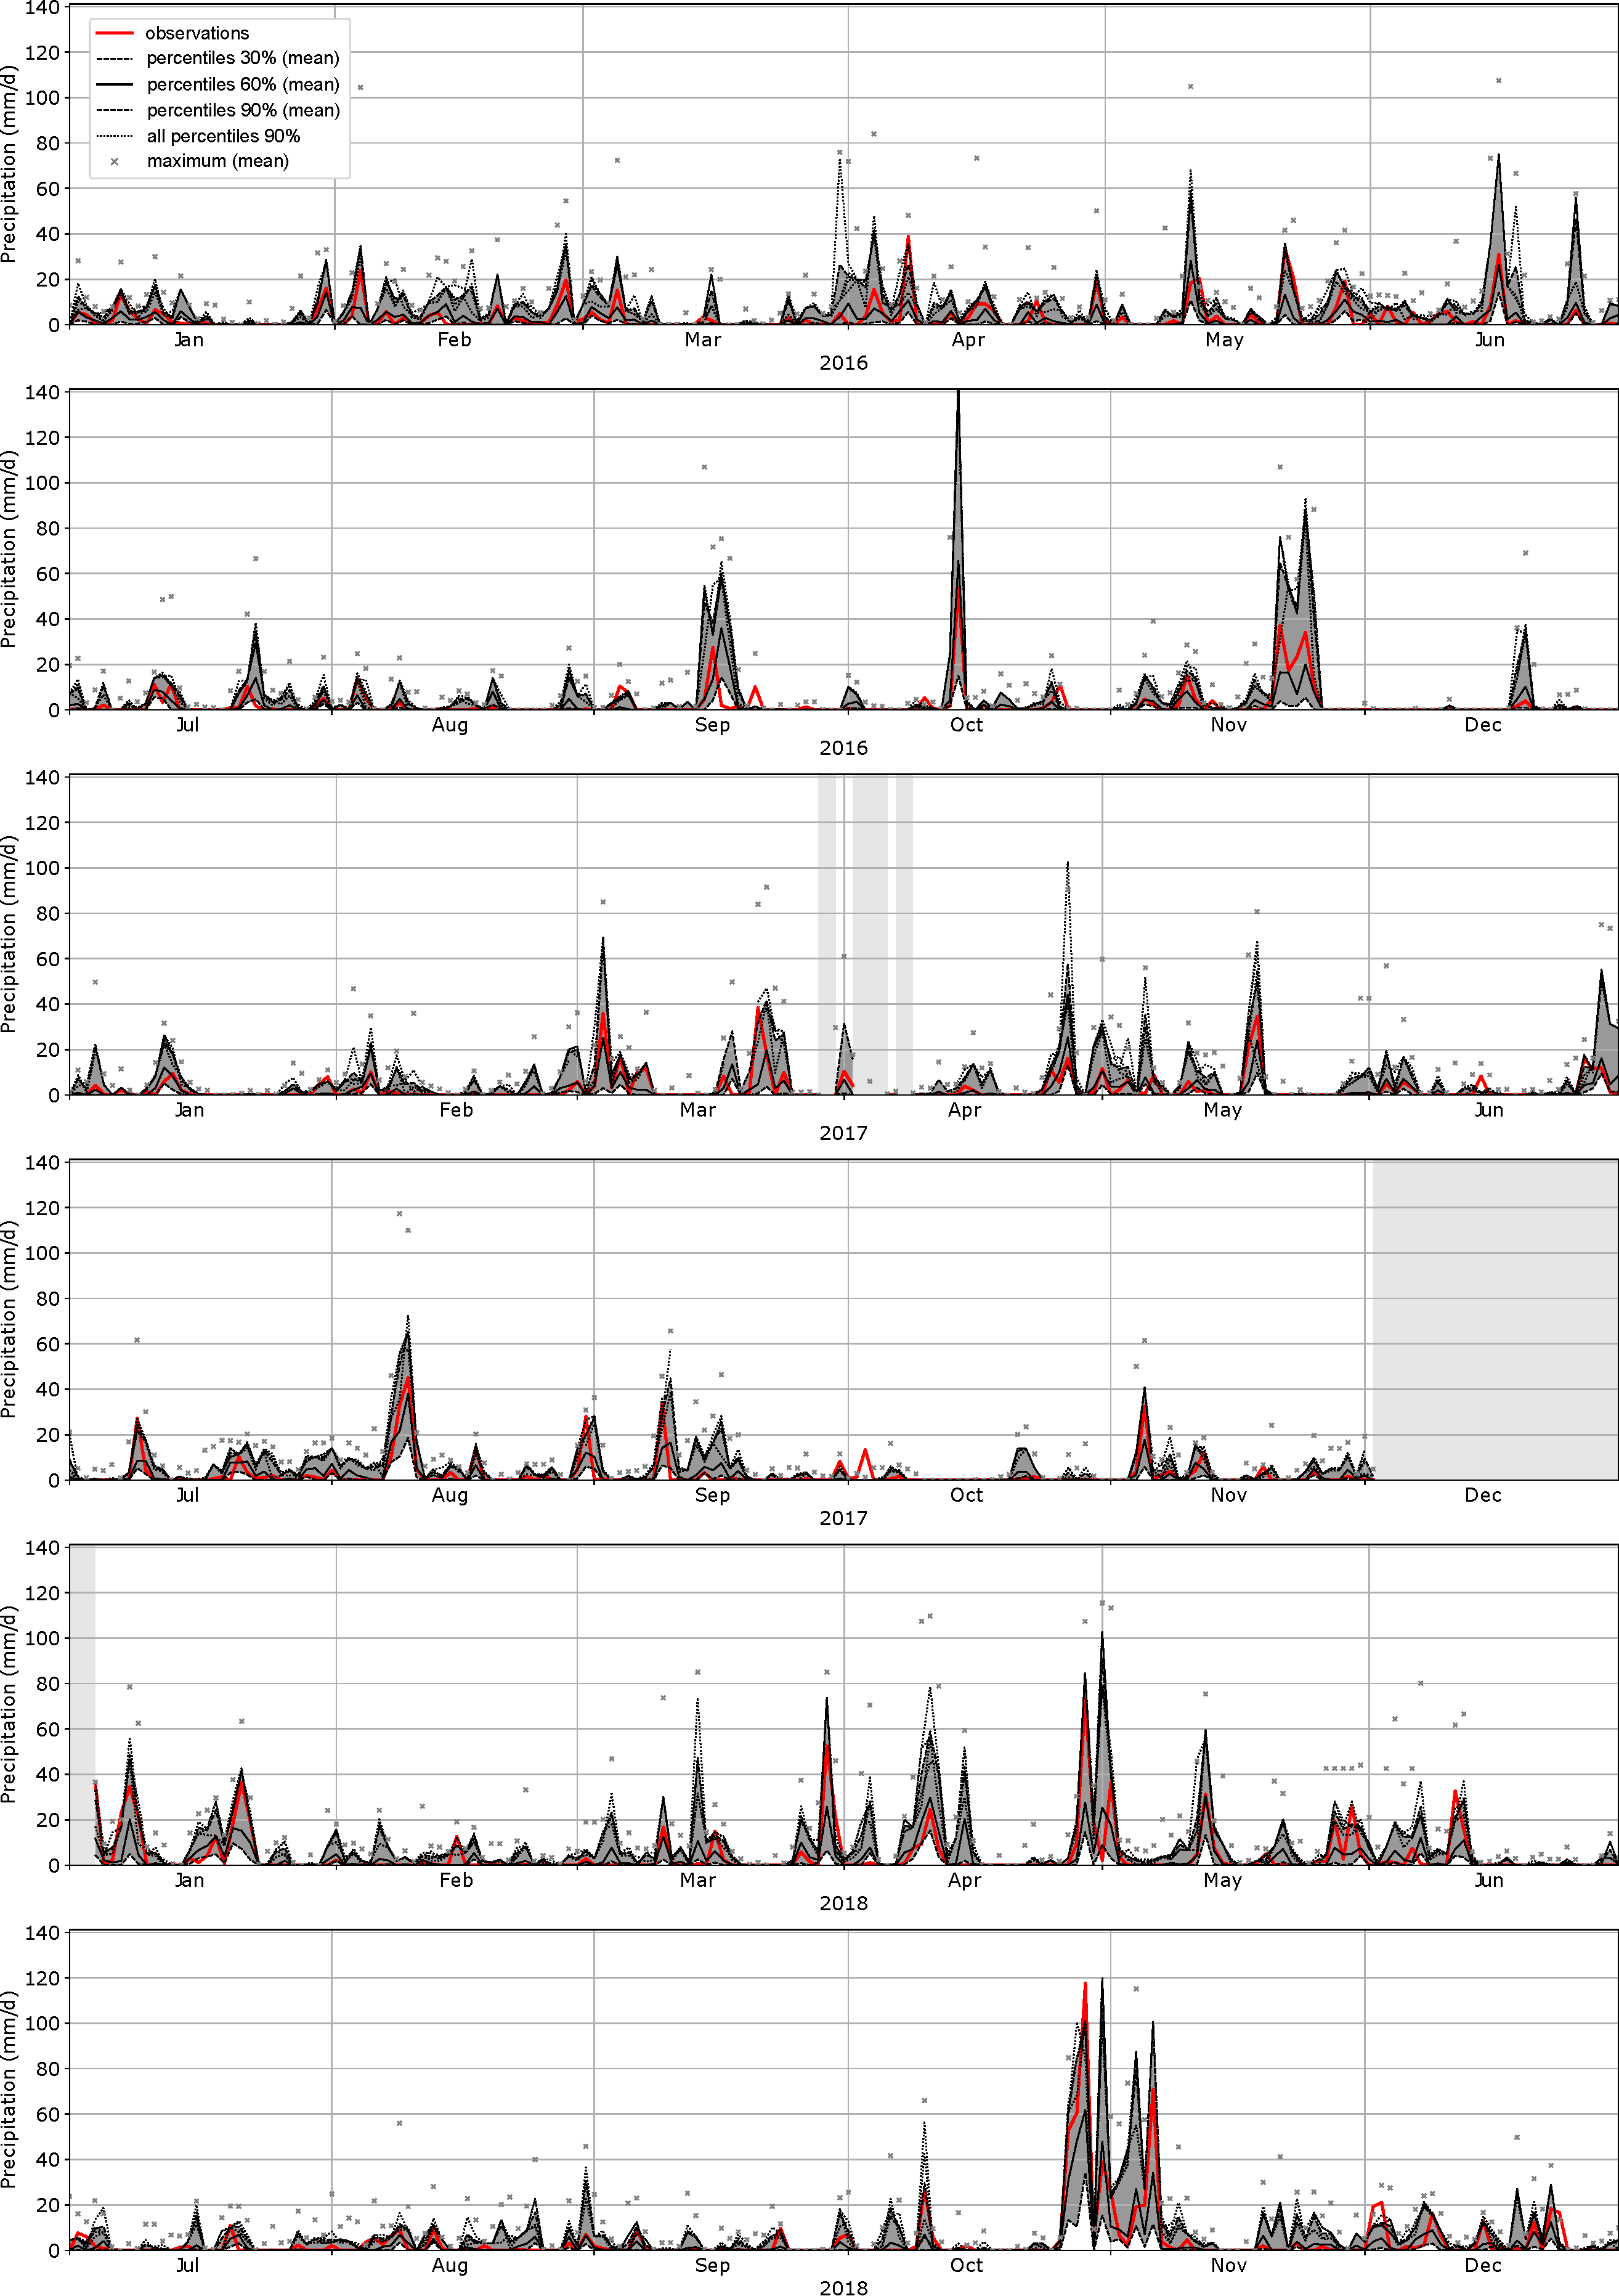
\includegraphics[width=16cm]{figures/fig_11.pdf}
	\caption{Forecasts for the Binn station (Fig. \ref{figure:variable_exploration}) over the period 2016--2018 obtained using the 4Zo method (Table \ref{table:methods}) with a lead time of three days. The distributions provided by the analog values are summarized by the $90^{th}$, $60^{th}$, and $30^{th}$ percentiles, as well as the maximum (crosses), all of them averaged over the four daily forecasts. Additionally, the four $90^{th}$ percentiles were also plotted to show the consistency / variability between the four daily forecasts. The shaded areas correspond to forecasts downtime.}
	\label{figure:operational_4z}
\end{figure*}

\begin{figure*}[hbt!]
	\vspace{-70pt}
	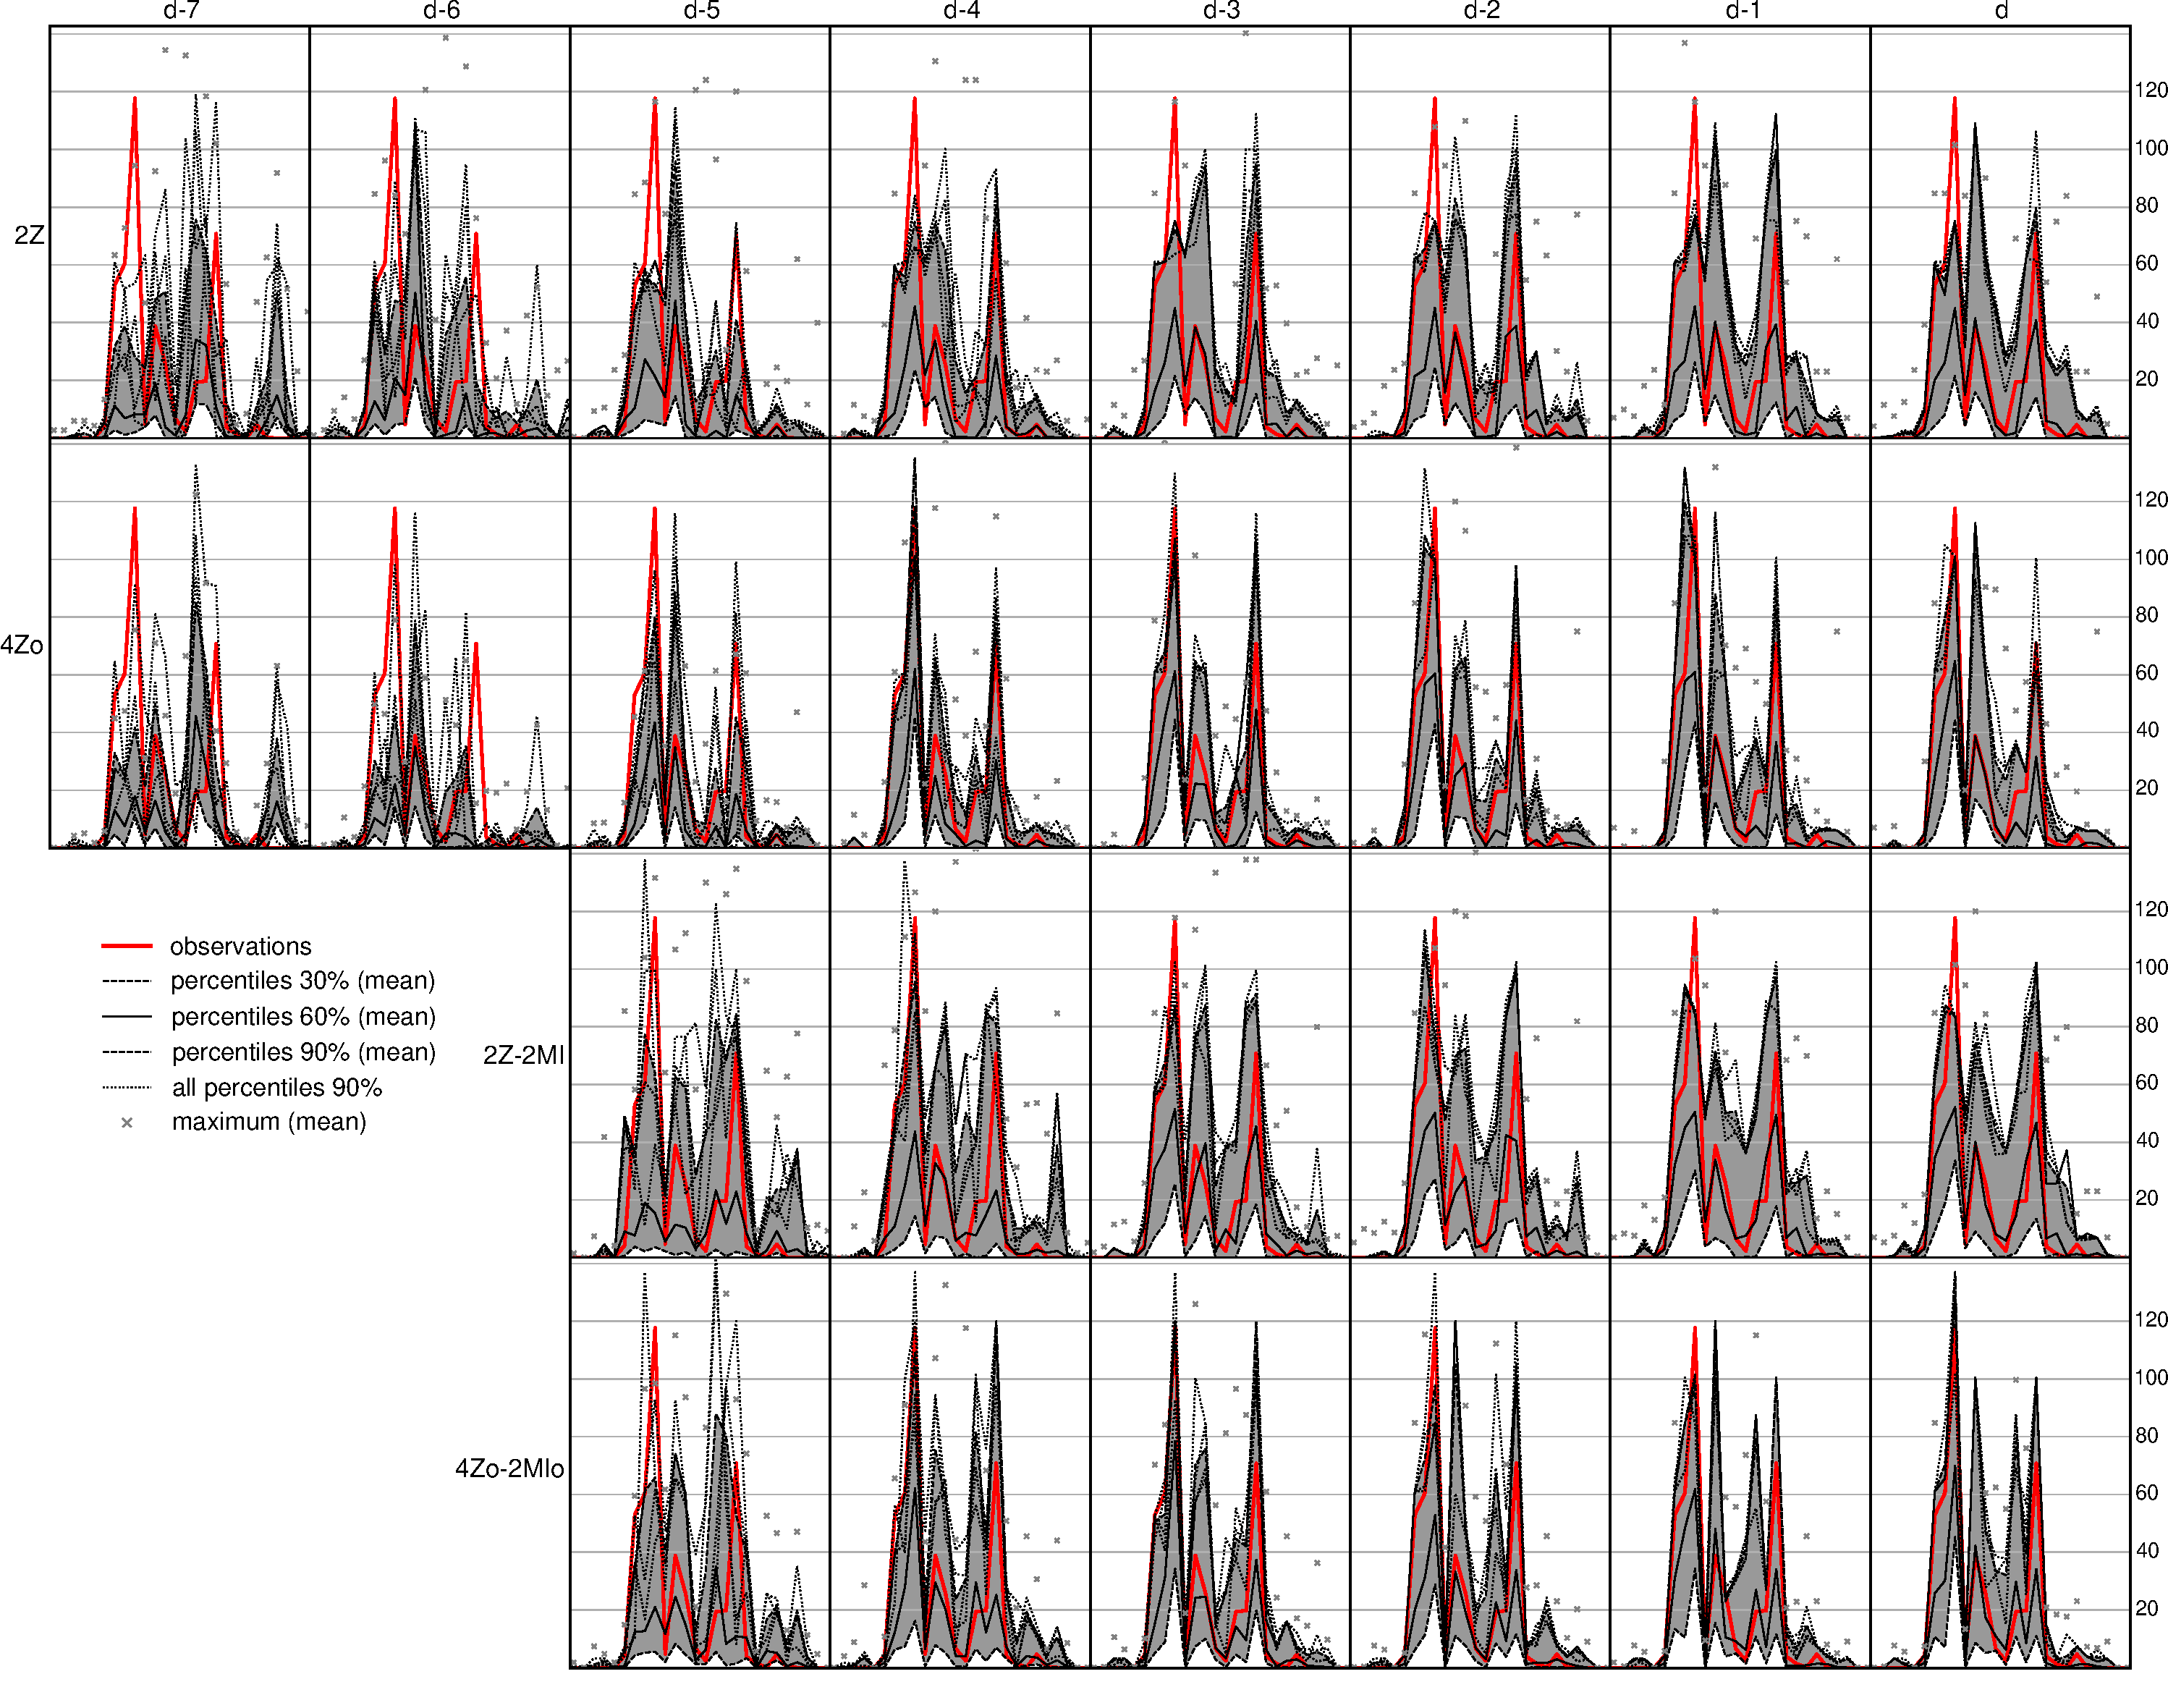
\includegraphics[width=16cm]{figures/fig_12.pdf}
	\caption{Same as Fig. \ref{figure:operational_4z_2mi} but for the 4Zo-2MIo method (Table \ref{table:methods}) with a lead time of one day.}
	\label{figure:operational_4z_2mi}
\end{figure*}

AtmoSwing Forecaster has been issuing operational forecasts since 2012 for the upper Rh\^one catchment in Switzerland (Fig. \ref{figure:variable_exploration}) in the context of a flood management project \citep{GarciaHernandez2009b}. First, the 2Z and 2Z-2MI methods were implemented using NR-1 as the archive and GFS outputs to describe the target situation \citep{Horton2012a}. Two more recent methods that were optimized by genetic algorithms \citep{Horton2018a} were also implemented since 2016. These methods were found to provide better results both in the perfect prognosis context and in the operational forecast. The results of the forecasts are provided for the Binn station (as in Sect. \ref{sec:parameters-space}) for the 4Zo method with a lead time of three days (forecast issued three days before the target day; Fig. \ref{figure:operational_4z}) and the 4Zo-2MIo method with a lead time of one day (Fig. \ref{figure:operational_4z_2mi}). For both methods and both lead times, the forecast obtained by analogs is satisfactory with observations falling within the distribution provided by the analogs. Moreover, when the analog distribution reached high values, it often matched with the observed high precipitation values. As discussed in Sect. \ref{sec:viewer}, high precipitation events are better described by the 90$^{th}$ percentile than the center of the distribution. The distributions provided by the analogs are quite large but nevertheless provide useful information.


Figure \ref{figure:operational_2018} shows how the most significant event (Oct./Nov. 2018) is predicted by the four implemented methods at different lead times. The two older methods (2Z and 2Z-2MI) do not forecast the main peak as well as the optimized ones (4Zo and 4Zo-2MIo). The forecast with a lead time of seven days show that high precipitation amounts can be expected, but the timing is not well defined as the four daily forecasts show high variability of the timing of the occurrence of the peaks (illustrated by the four forecasted 90$^{th}$ percentiles in Fig. \ref{figure:operational_2018}). The timing and amplitude of the event are relatively well captured by the 4Zo method with a lead time of four days. For the same lead time, adding moisture data (4Zo-2MIo) is not informative as the distributions are wider, and thus the occurrence of the peaks is more uncertain. Globally, moisture data was not very informative for this event. This might be related to the use of NR-1 as the archive, which has a very coarse resolution and was shown to not perform as well as other reanalyses \citep{Horton2018b}. It is likely that another dataset would be more accurate, and would be recommended for operational use.

\begin{figure*}[hbt!]
	\includegraphics[width=19cm]{figures/fig_13.pdf}
	\caption{Forecasts for the Oct./Nov. 2018 event at the Binn station (Fig. \ref{figure:variable_exploration}) for 2Z, 4Zo, 2Z-2MI and 4Zo-2MIo for lead times from seven to zero days prior to the target day.}
	\label{figure:operational_2018}
\end{figure*}
\clearpage

\section{Limitations of AMs}
\label{sec:limitations}

Although AMs were found to be relevant for several applications, they have some limitations which must be considered. The first is their lower performance for summer compared to winter \citep{Bliefernicht2010}. The relationship between synoptic predictors and local rainfall is lower in the summer, due to convective precipitations that present higher spatial variability and depend on other parameters. The variables that describe the synoptic circulation are indeed not able to predict the location of thunderstorm cells. This was also observed by \citet{BenDaoud2010}, who set up a specific model for the summer months (June 15 to September 15).

Another limitation is the need for a long archive of the predictand variable, for example, precipitation. Without several decades of data, AMs cannot be used. An alternative for regions without long archives of station measurements can be using satellite-derived precipitation. Long predictor archives are also required, which is easily satisfied with reanalyses. These may not be perfect in terms of homogeneity, but several can be considered to be of sufficient quality \cite{Horton2018b}. Moreover, reanalysis data are available all around the world, which represent a great potential for AMs.

Then, there is also the issue that extreme events may be under-represented in the considered sample of analog situations. Indeed, in a limited weather archive, events with high return periods are not frequent, which can introduce a bias in the prediction. There are however techniques to correct for this bias \citep[see][]{Marty2010}. In order to produce new extremes, postprocessing of the distribution of analogs might be necessary, for example, by using a scaling based on a predictor variable. 

It is also legitimate to raise the question of the relevance of an approach based on archives of past situations in the context of climate change. Changes in circulation frequencies and the persistence of certain weather types \citep{Hewitson1996} can be accounted for by AMs that contain predictors that characterize atmospheric circulation. Thus, if the archive of weather events is long enough, it is reasonable to assume that a large part of future events is already represented, even those whose frequency will change under different climatic conditions \citep{Wetterhall2005}. Changes in moisture and temperature variables must be accounted for to correctly capture the climate change signals. \citet{Dayon2015} has demonstrated the transferability of certain AMs to future climate conditions.


\section{Conclusions and perspectives}
\label{sec:conclusions}

AMs are cost-effective techniques for downscaling local meteorological variables from large-scale predictors. They are used in the context of operational forecasting for flood management or hydropower production, or in a climatic context for climate change impact modeling or reconstruction of past meteorological conditions. 

AtmoSwing is a suite of tools that facilitate processing of multiple AM structures in a flexible and efficient way. It consists of four software: the Forecaster for operational forecasting, the Viewer for displaying the Forecaster outputs, the Downscaler for applying AMs in a climatic context, and the Optimizer to infer the relationship between predictors and predictands. AtmoSwing is written in C++, is open source and has been extensively tested.

Processing operational forecasts with AtmoSwing requires very low computing infrastructure (implementation is possible on a Raspberry Pi 3) yet it can yield useful information, such as early warning for high precipitation events in the case of an application to flood forecasting. Valuable results were obtained in a three-year-long operational forecast in the Swiss Alps. With the global availability of reanalyses, it can be applied to any region with a relatively long predictand time series. The predictors and the structure of the method can be adapted to the local meteorological processes and controlled through xml files. The connection with open access NWP models such as GFS is integrated into AtmoSwing and requires no prior processing. The Forecaster can be installed on a computer or a headless server and run automatically to issue a forecast as soon as new NWP outputs are available. The Viewer offers a user-friendly display of the forecasts, with different levels of synthesis and details. It first provides an overview of potentially critical situations (possibility of high precipitation at a station for a certain lead time) but also allows plotting of the details of the distributions provided by the selected analog dates.

The Downscaler allows the AMs to be used in a climatic context, either for climate reconstruction or for climate change impact studies. When used for future climate analysis, the user must pay close attention to the selected predictors, so that they are able to represent the climate change signal. This is a relatively new field of application of AMs, which was proven to be of interest.

The Optimizer implements different optimization techniques, such as the sequential approach, a Monte--Carlo simulation, and a global optimization technique. Inferring the statistical relationship between predictors and predictand is quite intensive in terms of processing, as it requires numerous assessment over decades. To this end, the Optimizer has been highly optimized in terms of computing efficiency and is parallelized over multiple threads. It scales well on a Linux cluster. This procedure is only required to infer the statistical relationship, which can then be used in forecasting or downscaling at a low computing cost. 

One possible key improvement to AtmoSwing Forecaster is a multi-models approach that relies on outputs from multiple global NWP models to better take into account the uncertainty of the NWP forecasts. Similarly, \citet{Thevenot2004} demonstrated the benefit of using ensembles from global NWP as input for the method. The implementation consists of combining the selected analog days associated with each of the members. The forecast on the ensemble was found to be more accurate than the deterministic control for a lead time of four days and more \citep{Thevenot2004}. 

AtmoSwing aims to facilitate implementation of AMs with different types of structure and various predictors while being computationally efficient with low computing requirements. It can be applied to different contexts, allowing them to be operational forecasting or climate impact studies. It is open source and will hopefully save future users some development time.


\section*{Software availability}

AtmoSwing is free and open source (CDDL license). It is developed under the Git distributed revision control, and the source code can be found at:

\begin{itemize}
	\item AtmoSwing \citep{Horton2018c}: https://github.com/atmoswing/atmoswing/
	\item AtmoSwing R tools \citep{Horton2018d}: https://github.com/atmoswing/tools-r/
	\item AtmoSwing Python tools \citep{Horton2018e}: https://github.com/atmoswing/tools-py/
	\item Homepage: http://www.atmoswing.org
\end{itemize}


\section*{Acknowledgements}
Thanks to Charles Obled and Michel Jaboyedoff for their valuable inputs during the development of AtmoSwing. Thanks also to Lucien Schreiber and Richard Metzger for their programming advice and to Renaud Marty for his active involvement in testing AtmoSwing against his code base.  

Calculations were performed on UBELIX (http://www.id.unibe.ch/hpc), the HPC cluster at the University of Bern. Precipitation time series were provided by MeteoSwiss. The NCEP/NCAR reanalysis was provided by the NOAA/OAR/ESRL PSD, Boulder, Colorado, USA, at http://www.esrl.noaa.gov/psd/. ERA-interim was obtained from the ECMWF Data Server at http://apps.ecmwf.int/datasets/. 



\bibliography{references}

\clearpage

	
\end{document}

